\chapter{METHODOLOGY}

This chapter will present the methodology of the study. It will describe the research design, setting, data-gathering procedures, and the planned design and implementation of the proposed system to ensure that the study will be conducted systematically and aligned with its objectives.

\section{Research Design}
\begin{figure}[H]
	\centering
	\caption{Modified Waterfall Model of SDLC}
	\label{fig:waterfall}
	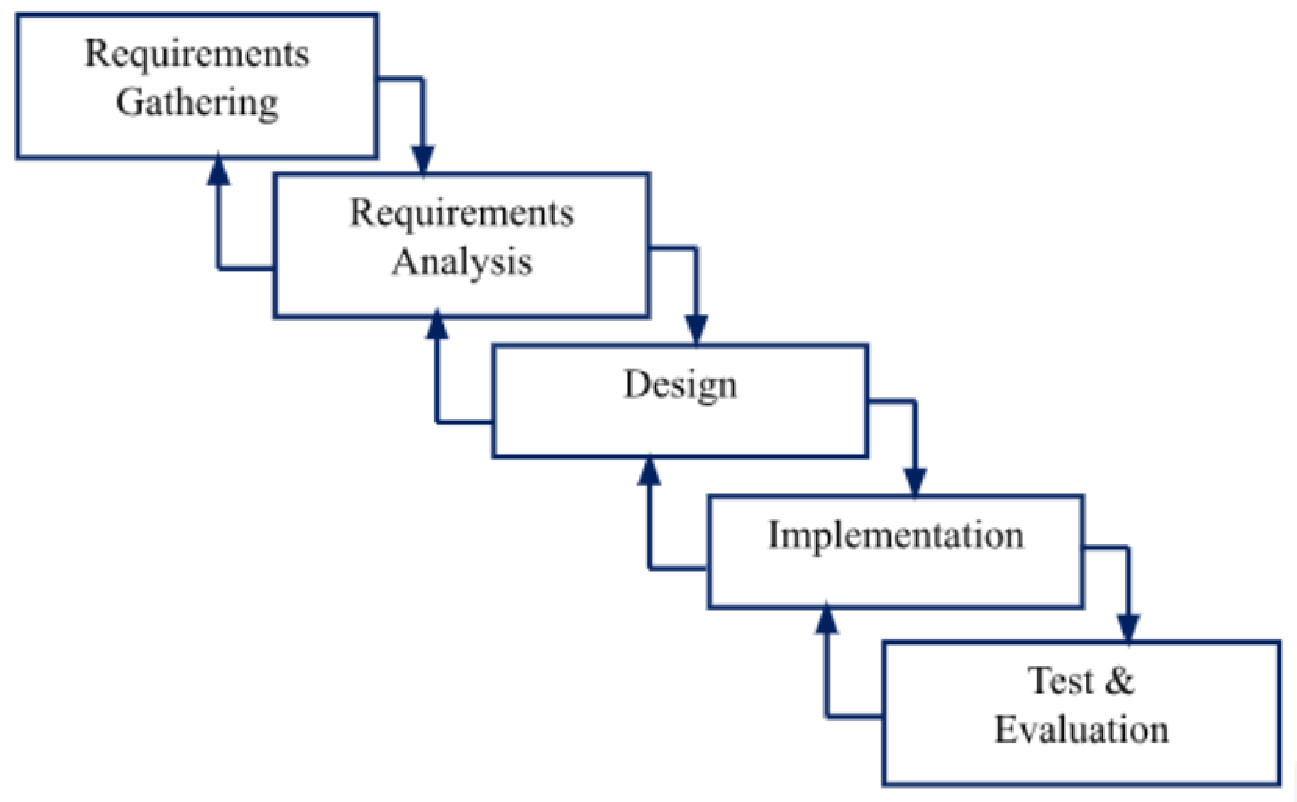
\includegraphics[width=0.9\textwidth]{figures/Waterfall.pdf}
\end{figure}

The methodology will be adopted from the Modified Waterfall Model of the Systems Development Life Cycle (SDLC). The methodology will be selected due to its structured yet flexible nature, allowing for sequential phases with opportunities for feedback and refinement. This will be particularly important in agricultural technology development, where both technical precision and field validation will be critical. For this study, it will enable the researchers to systematically design, implement, and evaluate the integration of UAV-collected imagery with YOLO for early disease detection in cacao pods, ensuring that each phase will be thoroughly reviewed before progressing to the next, while still accommodating necessary adjustments. Figure~\ref{fig:waterfall} shows the stages necessary for development.

\section{Research Setting}

\begin{figure}[H]
	\centering
	\caption{Janog Cacao Plantation in Initao, Misamis Oriental}
	\label{fig:cacao_farm}
	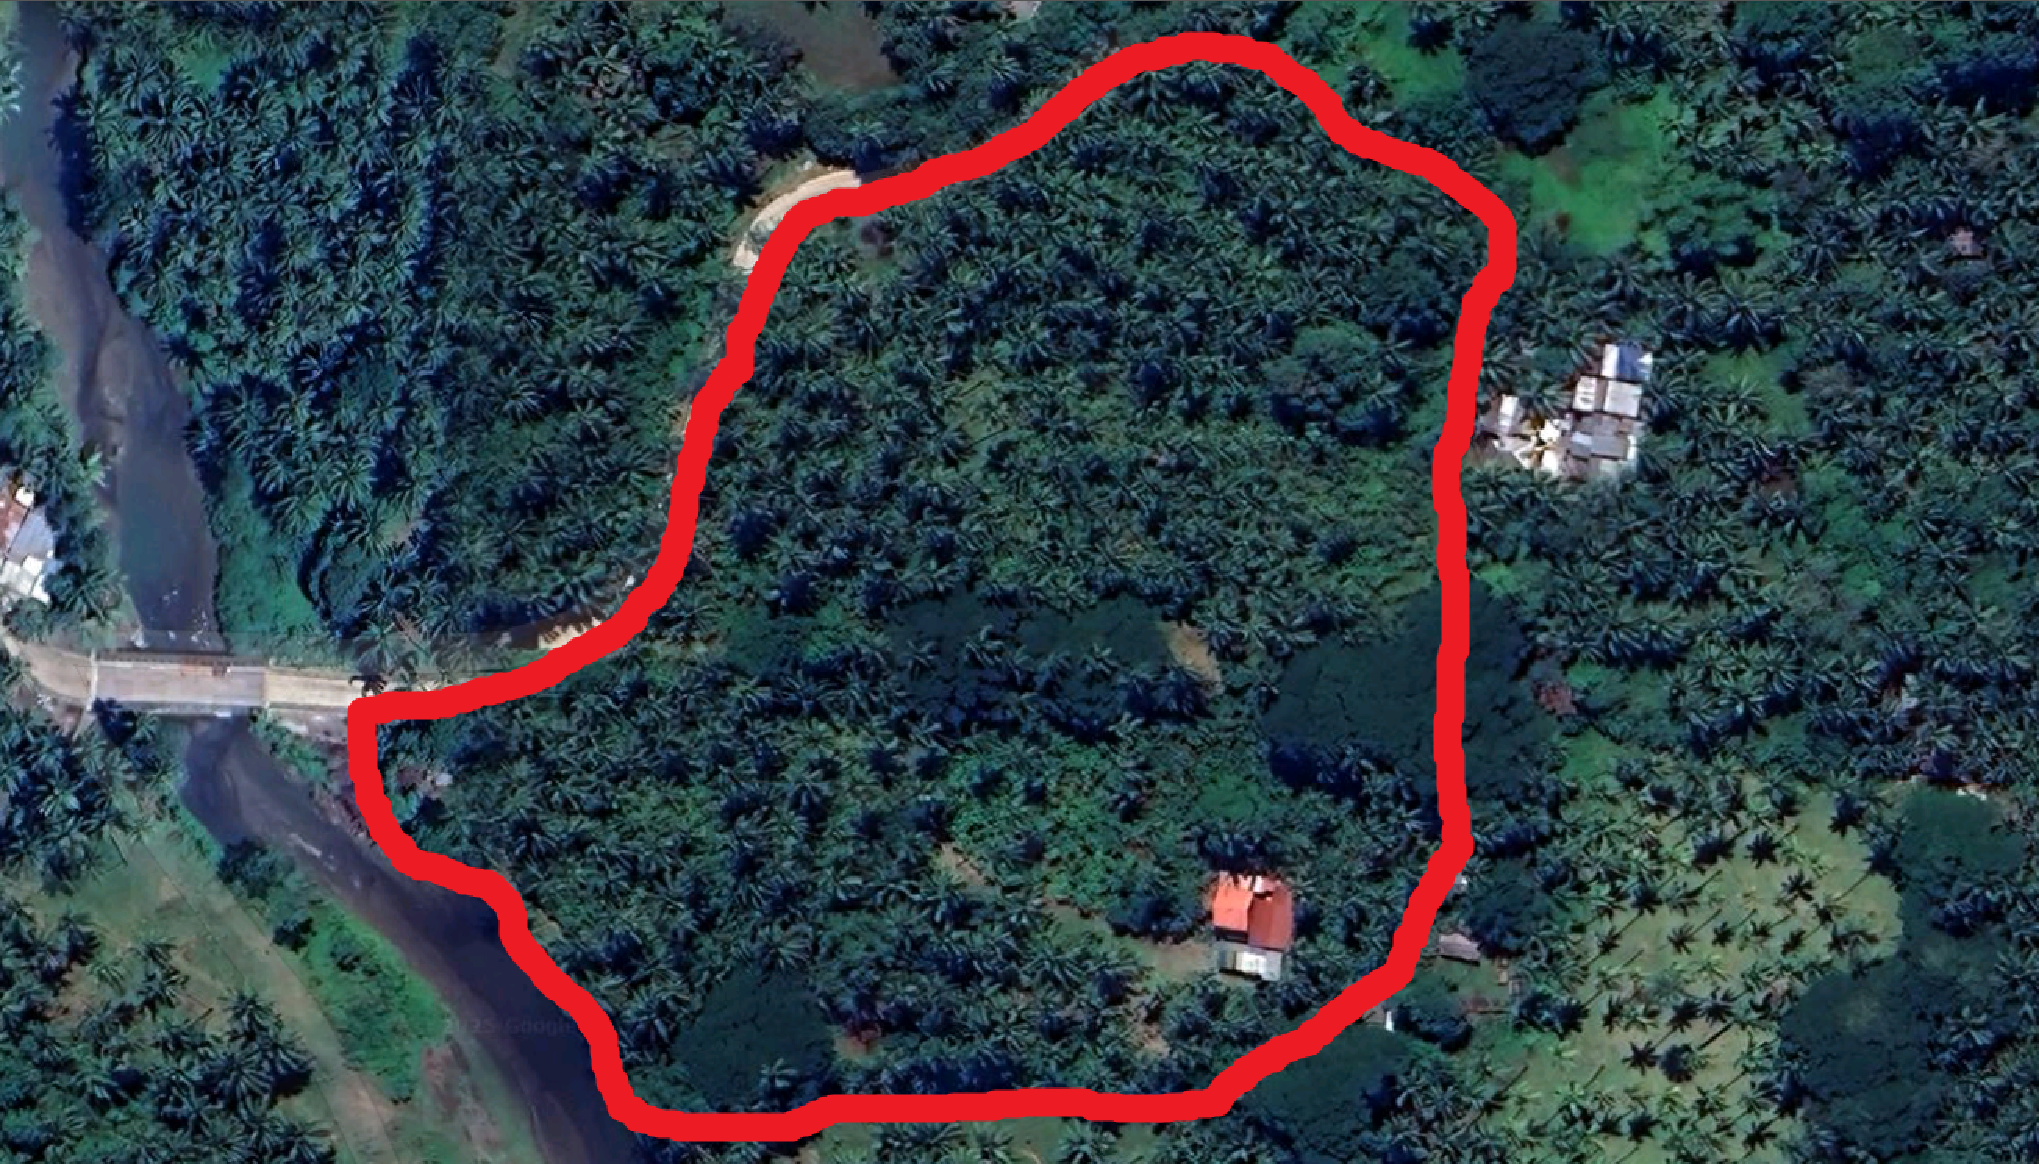
\includegraphics[width=1\textwidth]{figures/Cacao_Farm.pdf}
\end{figure}

Figure~\ref{fig:cacao_farm} shows the the location of the Janog Cacao Plantation in Initao, Misamis Oriental, which will serve as the research setting. 
The site is identified for its active cacao production and its relevance to the Philippine cacao industry, which continues to face significant challenges from black pod disease. 
The farm provides an appropriate real-world environment for implementing and testing the UAV-based detection system, as it represents typical small to medium-scale plantations in the region.

The farm environment contains multiple cacao trees arranged in rows, creating a suitable layout for structured UAV flights. 
This arrangement allows systematic data collection from varying altitudes and angles, ensuring that the captured images reflect diverse pod conditions, from healthy to infected. 

Farmers working in the area also serve as both observers and end-users, providing feedback on the practicality of UAV operations and the usability of the detection system.

The cacao planation in Initao is also identified for its accessibility to researchers while still representing rural farming conditions where advanced monitoring systems are rarely deployed. 
This balance makes the site ideal for testing the feasibility of precision agriculture tools in smallholder farm contexts. 
Ultimately, these factors make the cacao planation a practical and effective research setting for implementing and evaluating the proposed UAV-based cacao pod disease detection system.


\section{Research Setup}

The research setup utilizes a UAV (Unmanned Aerial Vehicle) equipped with a built-in high-definition camera and a GPS module to conduct low-altitude monitoring. The UAV flies at eye level, allowing it to capture detailed images of cacao pods directly from the side view of the trees.
This altitude ensures that the pods are recorded clearly, making it possible to identify early signs of black pod disease without the need for high-altitude aerial passes.

The UAV follows predefined paths along the rows of cacao trees to maintain systematic coverage of the plantation. 
Images are taken at regular intervals while moving at a steady pace, ensuring consistent data collection. 
Each image is automatically geotagged with precise coordinates provided by the integrated NEO-M8N GPS module. 
This process allows the researchers to later map infected pods within the farm using QGIS for visualization.

Since the UAV comes with a built-in imaging system, minimal hardware modifications are required. 
The programmable flight commands ensure repeatability in data collection, making the dataset reliable for training and validating the YOLO-based detection model.

\begin{figure}[H]
	\centering
	\caption{UAV Flight Paths in the Cacao Farm}
	\label{fig:uav_flight_paths}
	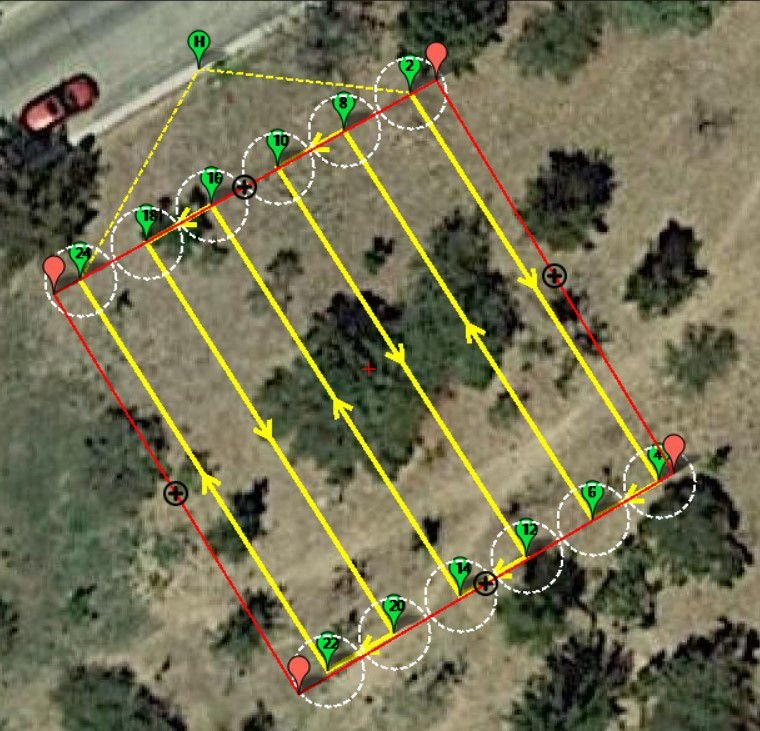
\includegraphics[width=0.9\textwidth]{figures/Uav_Flight_Paths.pdf}
\end{figure}

Figure~\ref{fig:uav_flight_paths} presents the UAV’s flight paths across the cacao farm. 
The drone moves parallel to the rows of cacao trees, ensuring overlapping coverage of pods and reducing blind spots. 
Flying at a low altitude provides close-range, high-resolution imagery of cacao pods, enabling accurate detection of visible symptoms of \textit{Phytophthora palmivora}. 
This approach minimizes issues related to lighting, wind, and stability while ensuring that the captured data is clear and consistent for system evaluation.



\section{Data Gathering}
To ensure a well-rounded and effective system design, data for this study will be collected from various relevant sources:

\subsection*{Sources of Data}
\textbf{Cacao Farmers and Field Personnel}. Surveys and interviews will be conducted with cacao growers and farm workers to gather insights on existing practices for disease detection, common issues encountered in the field, and expectations for a UAV-based detection system. Agricultural Specialists. Input agricultural professionals will be obtained to identify key disease symptoms, validate detection criteria, and provide guidance on effective monitoring strategies for cacao pod health.

\textbf{Existing Literature and Research Studies}. A comprehensive review of academic and technical literature, such as studies by Baculio \& Barbosa (2022), Vera et al. (2024), and Solpot (2020), will support the design of the detection system by offering benchmarks on accuracy, image processing, and the use of machine learning in agriculture.

\textbf{Technology Experts}. Consultations with UAV technicians, AI developers, and computer vision experts will be sought to ensure the system’s technological components such as image acquisition and model training are both feasible and optimized for agricultural environments.

\subsection*{Data Gathering Procedure}

To gather relevant data that will inform the design and development of the cacao pod disease detection system, this study will utilize both questionnaires and interviews.

\textbf{Questionnaire}. A structured questionnaire will be distributed to cacao farmers and field personnel to gather information about their current practices in detecting cacao pod diseases, the challenges they face in early identification, and their perspectives on using UAV-based solutions. Before distribution, the questionnaire will be reviewed and approved by the research adviser, agricultural specialists, and academic authorities to ensure that it is technically sound, ethically appropriate, and aligned with the objectives of the study.

\textbf{Interview}. Interviews will be conducted with cacao farmers, agricultural experts, plant pathologists, UAV technicians, and AI developers. These interviews aim to collect in-depth insights on disease symptoms, detection indicators, drone imaging strategies, and technical requirements for integrating YOLO into an agricultural setting.

\textbf{Existing Literature}. A review of relevant literature will be conducted to understand the current state of disease detection systems in agriculture, particularly focusing on cacao pod diseases. This will include studies on the use of UAVs, AI-driven disease detection models (such as YOLO), and the challenges associated with deploying such technologies in farming environments and provide a foundation for comparing the proposed system with existing solutions.

\subsection*{Data Finding Analysis}

To gather relevant data, this study will employ multiple data collection methods.

\textbf{Qualitative Analysis}. Thematic analysis will be applied to interviews and open-ended survey responses. This approach will help identify recurring themes such as difficulties in manual disease detection, trust in machine learning techniques, and challenges related to the adoption of UAVs. Insights from this analysis will inform user-centered system design and guide improvements in usability and functionality.

\textbf{Quantitative Analysis}. Descriptive statistical analysis will be used for the structured survey data. This includes calculating frequencies, percentages, and average values to measure levels of technological readiness, prevalence of black pod disease, and the willingness of users to adopt UAV-based solutions for monitoring. These metrics will provide measurable indicators to support system feature prioritization.


\textbf{Feasibility Analysis}. Sensor specifications and machine learning model performance will be assessed through expert consultations and a review of relevant literature. This includes evaluating the accuracy of YOLO for disease detection and the practicality of drone operation in cacao farm environments using a performance matrix.

\textbf{Spatial Analysis}. Given that the UAV system captures geo-tagged images, spatial analysis will be conducted to examine the geographical distribution of detected disease cases. This analysis will help visualize infection hotspots across the farm and support precision intervention strategies. Tools such as heatmaps or geospatial clustering may be used to map and interpret disease spread over time and space.

\section{Requirement Gathering}

This section presents the requirements gathering conducted by the researchers. The data were collected through an interview with a local cacao farmer who has extensive experience in cacao production and management. The purpose of this interview was to understand the existing farming practices, challenges in disease detection and management, and collect essential information for system development. 

Before the engagement, the researchers prepared a set of open- and closed-ended questions to guide the discussion. A consent letter outlining the ethical use of the collected information was also presented to the respondent, ensuring that all gathered data would be used solely for academic and research purposes in compliance with data privacy regulations. (Refer to Appendix B) 

The respondent has been cultivating cacao for nine (9) years and manages a farm covering approximately five (5) hectares with more than 2,500 cacao trees planted at a spacing of three (3) meters per tree. The farm contains various elements, including tall coconut trees that provide shade, nearby power lines, and a river, none of which significantly affect the farm’s operations. The farmer personally inspects the cacao pods on foot, as this is currently the only available method to monitor the trees for pest infestations and diseases.

According to the respondent, major challenges in cacao farming include high costs and labor-intensive practices, particularly in spraying, pruning, and pest control. However, the most critical issue arises during the rainy season, as it contributes to the spread of Phytophthora, the fungus responsible for black pod rot, locally referred to as butikol. During these periods, only about one (1) out of every ten (10) trees remains healthy, and the number of harvestable pods varies significantly depending on weather conditions.

The farmer identifies diseased cacao pods primarily through their appearance, observing signs such as discoloration and the presence of small dark dots, which are associated with Phytophthora infection. Once symptoms appear, even at an early stage, the affected pods are immediately removed to prevent further contamination of nearby fruits. Although spraying is conducted as a preventive measure, some infected pods remain unnoticed due to the vast area of the farm and the intensity of labor required.

Farm inspection is done daily, taking approximately three (3) weeks to complete a full cycle across all areas of the farm. The farmer increases inspection frequency during the rainy season, as losses are significantly higher compared to the dry season. Fertilizers are also applied for quality control, with an estimated expenditure of thirty thousand pesos (₱30,000) per cycle.

During the peak harvest season, typically from November to December, the farm produces around 300 to 500 kilograms of cacao beans, which are sold to vendors from Davao at a price of ₱300 per kilogram. However, yields lower than 200 kilograms are considered a deficit. Based on the respondent’s estimate, approximately twenty (20) pods are required to produce one (1) kilogram of beans. The pods vary in color red to orange, and green to yellow with yellow pods indicating ripeness. Harvesting and pruning are performed manually using pruners or saws, with extra care taken to avoid damaging the fruit-bearing branches. (see Appendix D)


\subsection*{User Definition}

Following the requirements gathering process, the primary user of the system has been identified.

\textit{Farmers} - The primary user of the system, responsible for utilizing UAVs to detect early signs of cacao pod diseases and making informed decisions for crop management.

\begin{longtable}{p{4cm} p{8cm}}
	\caption{System Requirements} \label{tab:sysreq}                                                                                                                                      \\

	\toprule
	\textbf{Category}        & \textbf{System Requirements}                                                                                                                               \\
	\midrule
	\endfirsthead

	\toprule
	\textbf{Category}        & \textbf{System Requirements}                                                                                                                               \\
	\midrule
	\endhead

	\bottomrule
	\endfoot

	Input Requirements       & - The system shall collect images of cacao pods captured by UAVs for disease detection.                                                                    \\
	                         & - The system shall allow users to initiate UAV image capture and review sessions through a simple interface.                                               \\
	                         & - The system shall utilize annotated image datasets for training the AI model, specifically focusing on black pod disease.                                 \\
	                         & - The system shall use GPS metadata from UAVs as input to geo-tag disease detection results.                                                               \\
	\midrule

	Process Requirements     & - The system shall process captured images using the YOLO model to identify and classify diseased cacao pods.                                              \\
	                         & - The system shall preprocess input images for consistency.                                                                                                \\
	                         & - The system shall utilize a labeled image dataset of cacao pods.                                                                                          \\
	                         & - The system shall include a manual annotation process where images are labeled with infection presence and location.                                      \\
	\midrule

	Output Requirements      & - The system shall display detection results, highlighting infected areas on cacao pods in real-time or after processing.                                  \\
	                         & - The system shall classify each detected pod as either healthy or infected.                                                                               \\
	                         & - The system shall provide GPS coordinates alongside detection results for mapping infected areas.                                                         \\
	                         & - The system shall generate summary reports including: total number of pods detected, number and percentage of infected pods, detection time and location. \\
	\midrule

	Control Requirements     & - The system shall implement secure access with user authentication to ensure that only authorized users (farmers) can access the system.                  \\
	                         & - The system shall maintain logs of image captures, analysis sessions, and user feedback for audit and traceability.                                       \\
	                         & - The system shall validate all image inputs and user entries to ensure accurate and usable data is processed.                                             \\
	\midrule

	Performance Requirements & - The system shall be capable of processing high resolution images in real-time or near real-time with minimal latency.                                    \\
	                         & - The system shall efficiently manage and store large datasets of images and detection results, supporting scalable usage over time.                       \\
	                         & - The system shall maintain uptime and availability to ensure uninterrupted use during farming operations.                                                 \\
\end{longtable}

\section*{Design and Implementation}

\subsection*{System Architecture}

\begin{figure}[H]
	\centering
	\caption{System Architecture of the Study}
	\label{fig:SysArch}
	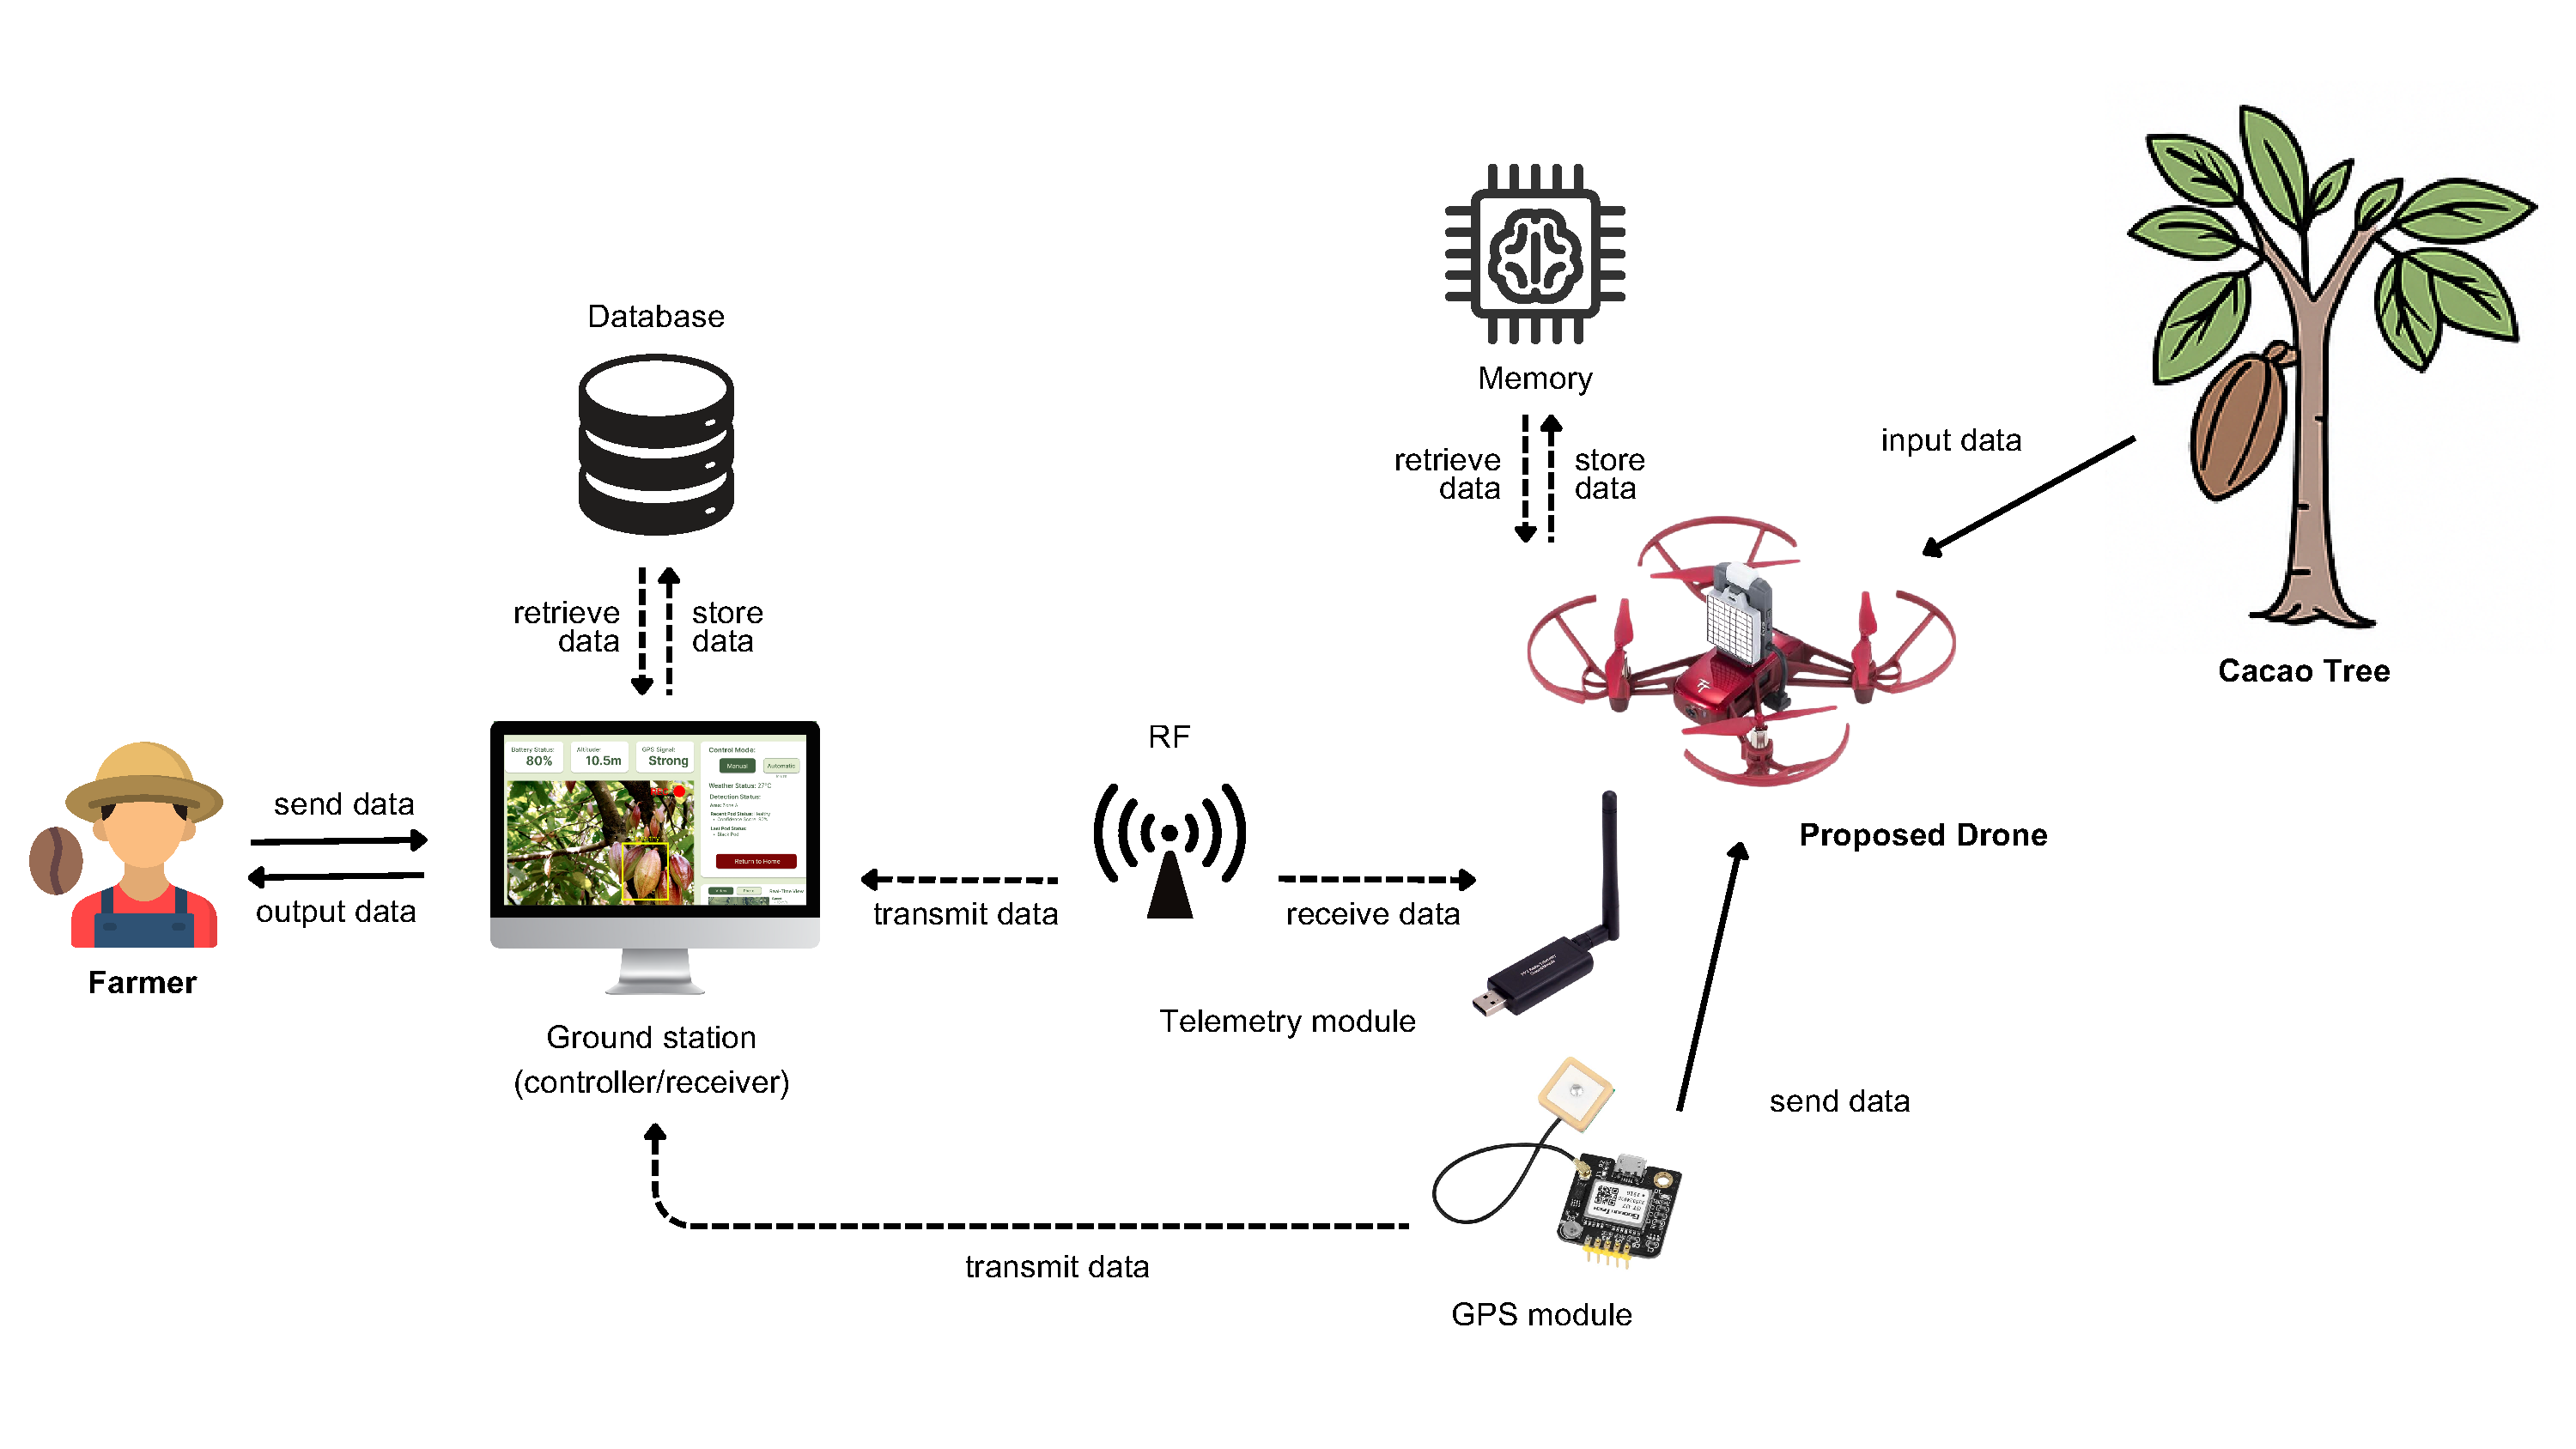
\includegraphics[width=0.9\textwidth]{figures/Sys_Arch.pdf}
\end{figure}

Figure~\ref{fig:SysArch} illustrates the system architecture of the study. The process begins with the cacao trees, which are the central focus of the system. To monitor them, a proposed drone is deployed over the farm. This DJI RoboMaster TT is equipped with cameras and sensors that collect input data—primarily images and environmental readings—from the trees as it flies at the same level as them. The data captured by the drone is transmitted to an open-source controller with a camera module, which acts as the drone’s mini computer. This device processes the incoming images and sensor data. Additionally, a GPS module connected to the system sends precise geolocation data to the processor, tagging the collected images with accurate coordinates. Once the data is processed, it is temporarily stored in a memory unit. From there, the data is transmitted using a telemetry module, which serves as a bridge between the drone and the ground systems. The telemetry module sends the data wirelessly via RF to the web-based system, which acts as both a controller and a receiver. It receives the telemetry data and displays it in a user-friendly format, allowing the farmer to monitor the status of the cacao trees. The farmer can also send commands or control inputs back to the system using the system. All this information can be stored and retrieved from a database for later analysis or reference. The farmer is empowered with clear insights about the farm’s condition without needing to be physically present at each tree.

\subsection*{Flowchart of Hardware and Software}

\begin{figure}[H]
	\centering
	\caption{Hardware Flowchart}
	\label{fig:HardFlow}
	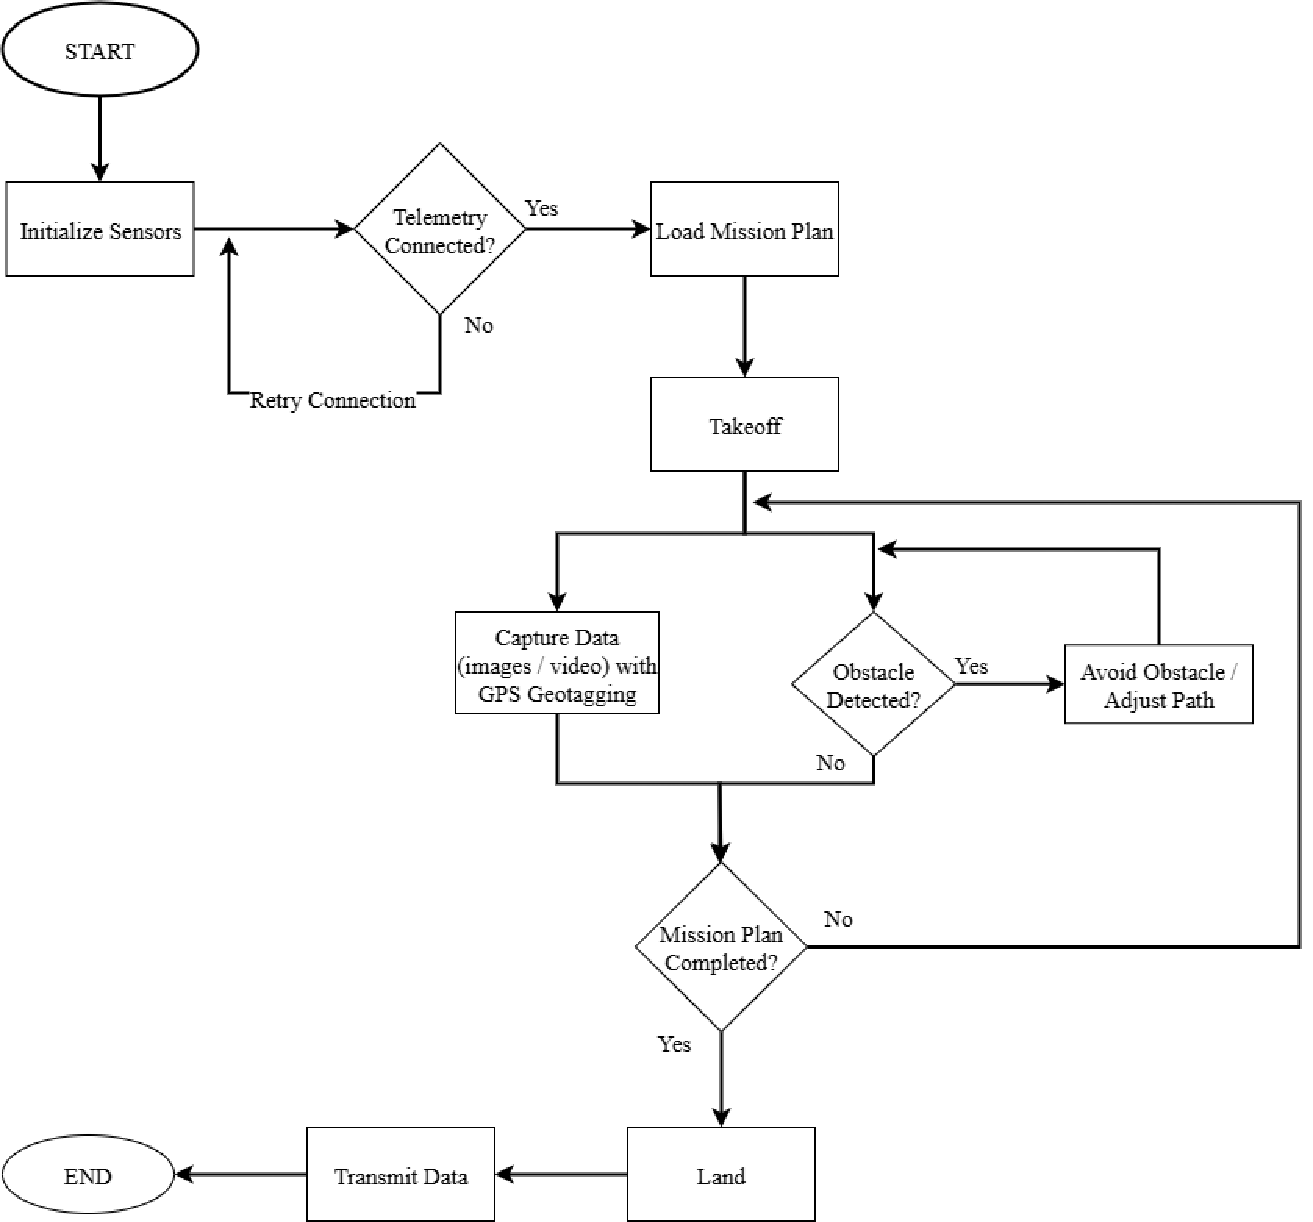
\includegraphics[width=0.9\textwidth]{figures/Hard_Flow.pdf}
\end{figure}

Figure~\ref{fig:HardFlow} illustrates the operational workflow of the UAV system; it begins with powering on the UAV, followed by the initialization of its key sensors, including the camera, GPS module, and obstacle detection system. Once the sensors are active, the system checks for telemetry connectivity with the ground station; if the connection fails, the drone retries until successful. After establishing a link, the mission plan is loaded from the ground station, and the UAV proceeds to takeoff. During flight, two processes run in parallel: the drone continuously captures images and videos with GPS geotags for later processing, while simultaneously monitoring its environment for obstacles and adjusting its path when necessary. The system then checks whether the mission plan has been completed. If it is complete, the UAV proceeds to land; if not, it continues executing the remaining tasks until completion. Only after landing are the stored image and location data transmitted to the ground station for processing. The operation then concludes with system power down.

\begin{figure}[H]
	\centering
	\caption{Software Flowchart}
	\label{fig:SoftFlow}
	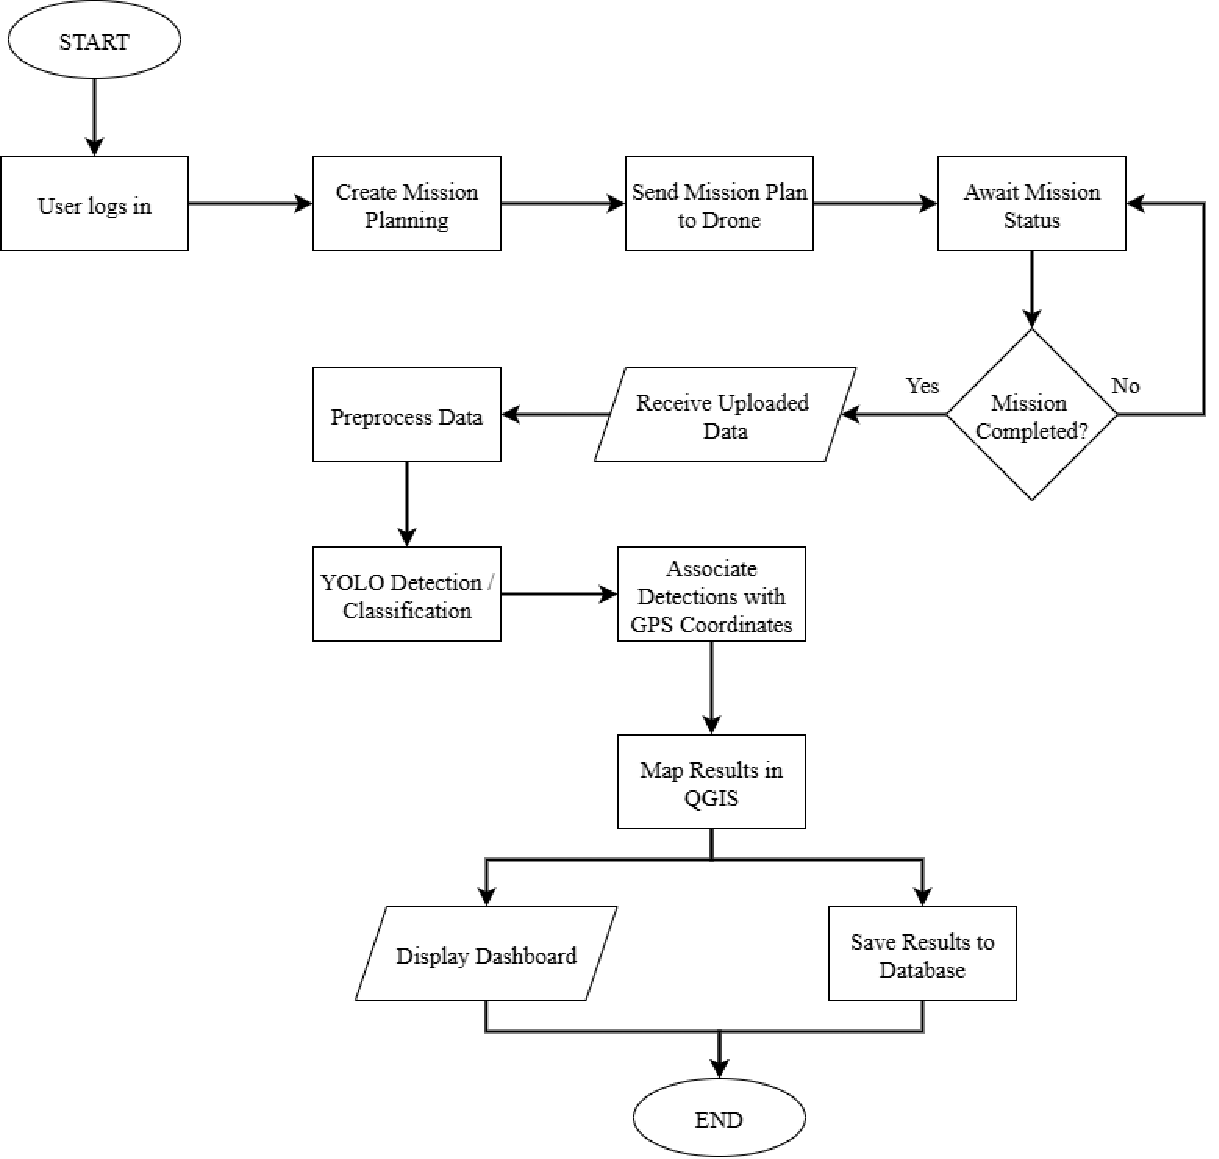
\includegraphics[width=0.9\textwidth]{figures/Soft_Flow.pdf}
\end{figure}

Figure~\ref{fig:SoftFlow} shows the software workflow, starting with the user logging into the system and creating a mission plan that defines waypoints, altitude, and capture intervals. This plan is then sent to the UAV through SDK, after which the system awaits mission status updates. At this stage, a decision point determines whether the mission has been completed. If the mission is successful, the system retrieves the uploaded images with their GPS metadata; otherwise, it continues waiting until completion. Once the data is received, the images undergo preprocessing such as resizing, normalization, and augmentation before being passed through the YOLO algorithm for disease detection and classification. The detection results are then associated with GPS coordinates to ensure spatial accuracy and are mapped in QGIS to generate a clear visualization of affected areas. From this stage, two operations run in parallel: results are displayed on the dashboard for immediate user insight, while the same results are saved into the database for reporting and long-term storage. Finally, the processes converge, and the mission concludes to complete the workflow.

\subsection*{Ground Station Architecture}

\begin{figure}[H]
	\centering
	\caption{Ground Station System Design and Workflow}
	\label{fig:GroundStation}
	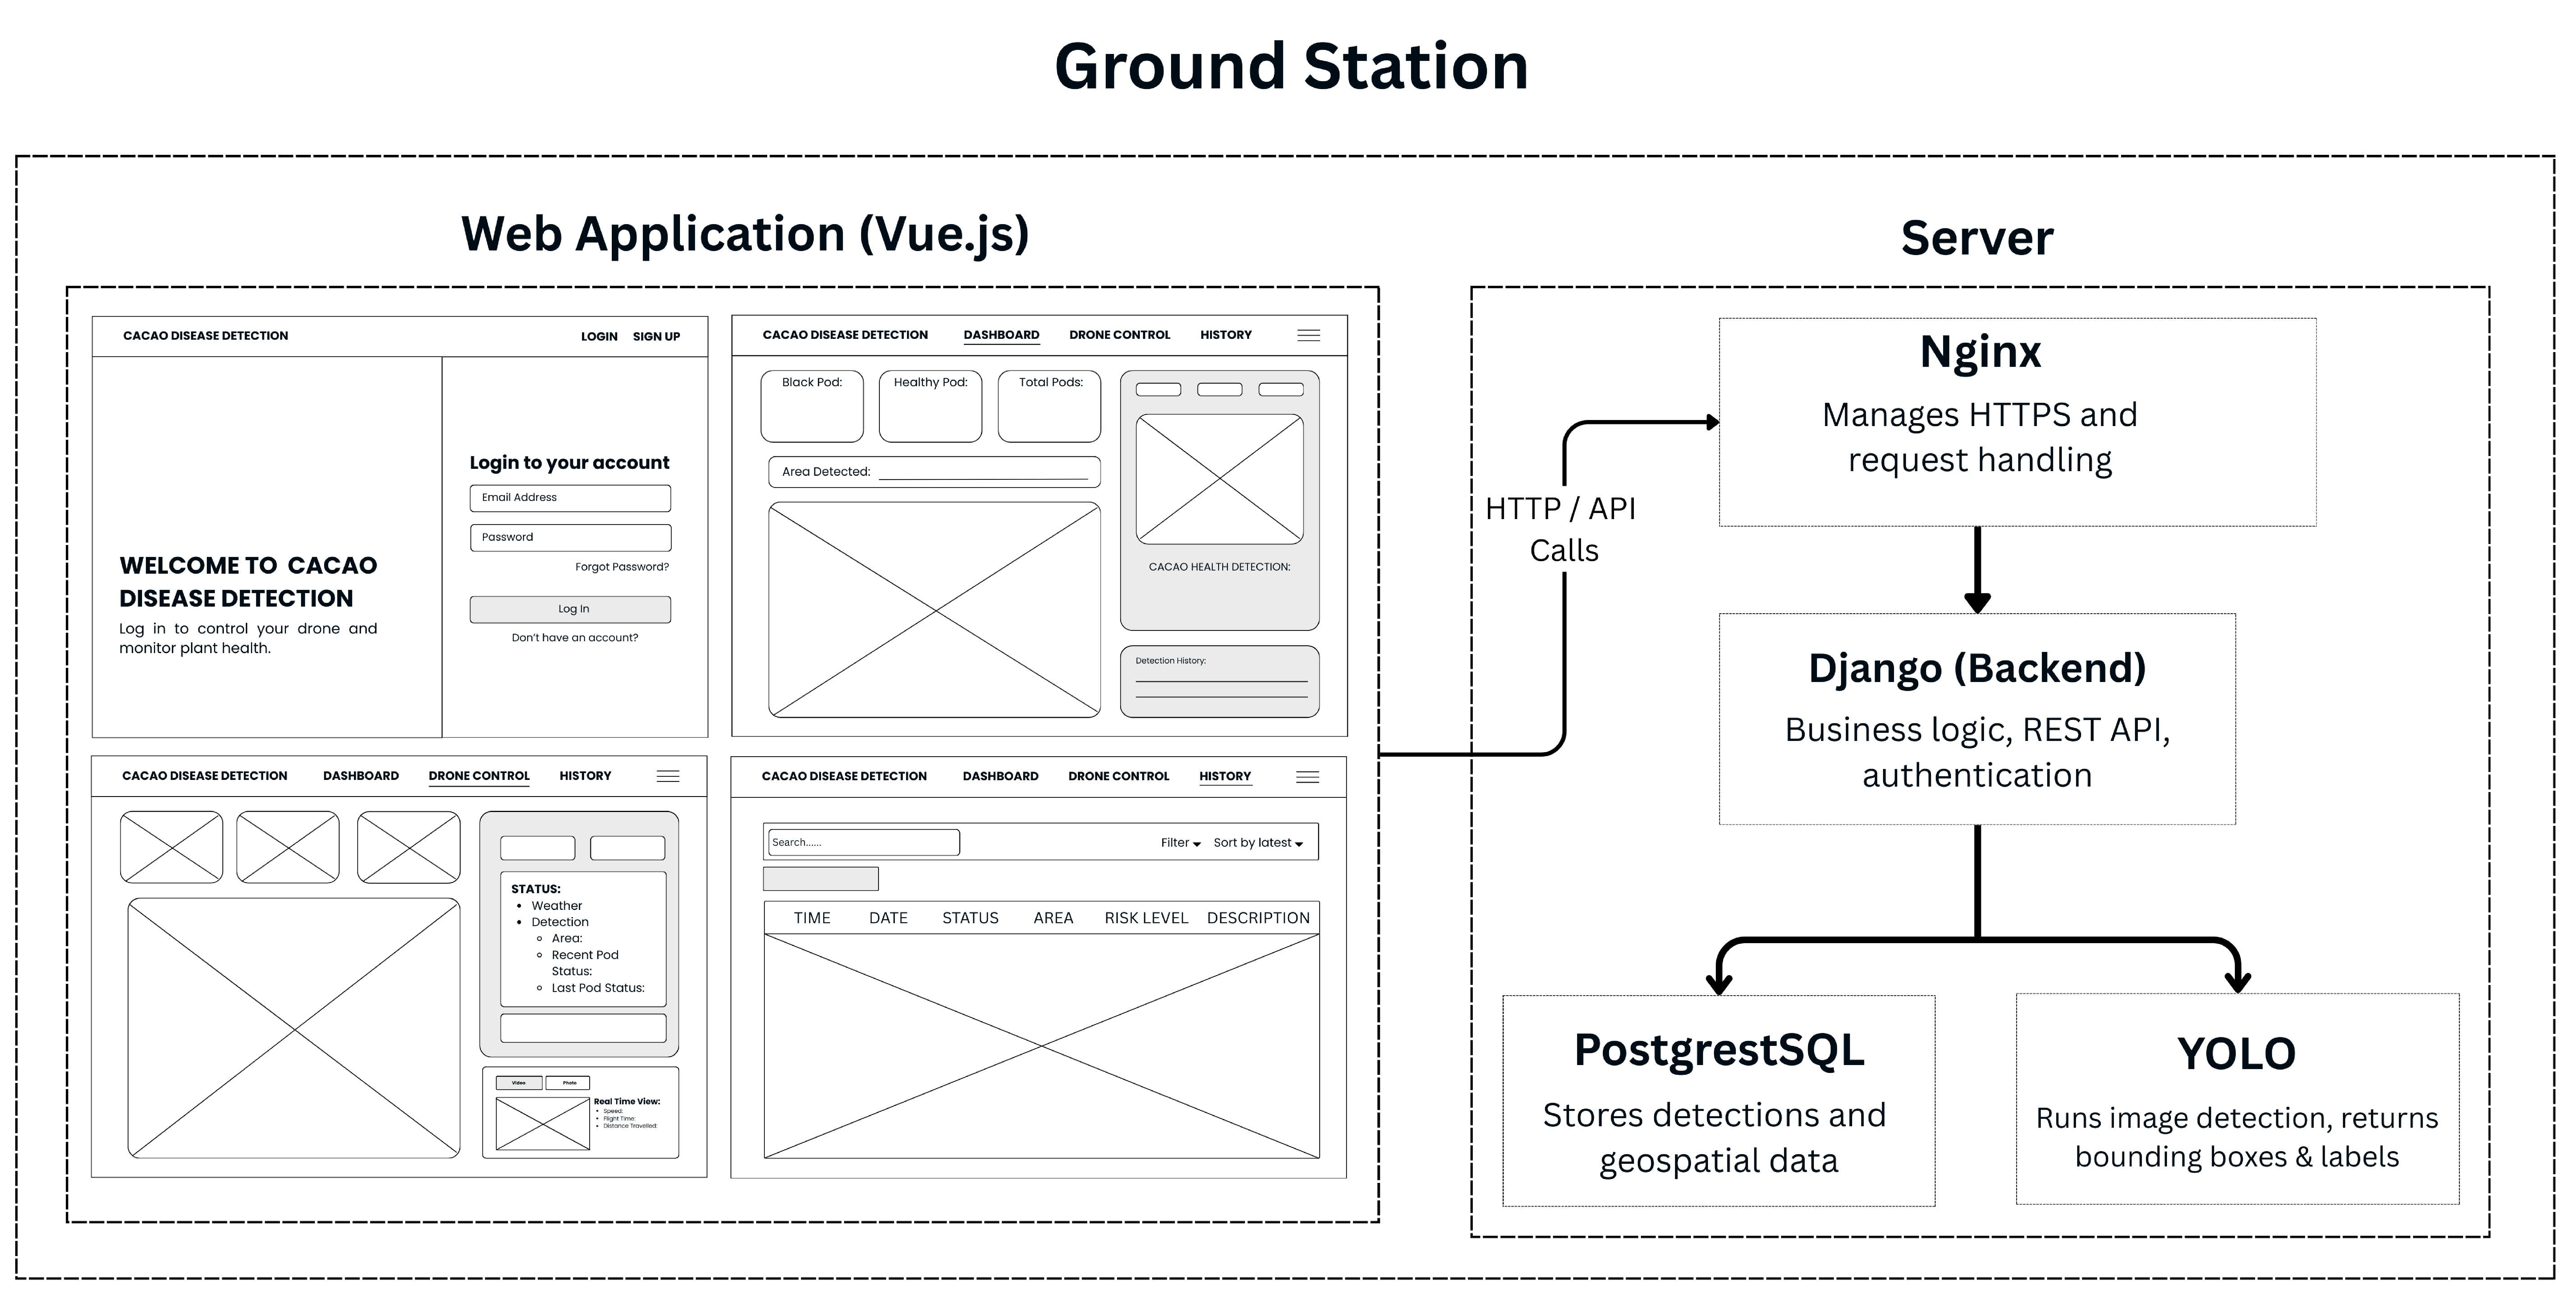
\includegraphics[width=1\textwidth]{figures/Ground_Station.pdf}
\end{figure}

Figure~\ref{fig:GroundStation} presents the entire system that manages the processing of UAV data and delivers results to the end user. It is composed of two closely connected parts: the web application and the server components.

The web application, developed in Vue.js, serves as the main interface for users. It provides modules for user authentication, drone mission control, and the visualization of detection outputs. The dashboard summarizes key statistics such as the number of pods identified as healthy or infected, while the history module allows users to review past detections and track trends over time. Through this interface, farmers are able to easily monitor the health of their crops and make informed decisions.

The server side of the Ground Station integrates several core technologies. Nginx acts as the web server and reverse proxy, handling HTTPS traffic and routing requests. Django functions as the application server, implementing the system’s logic, managing authentication, and exposing a REST API for the web application. The detection process is carried out by the YOLO module, which receives aerial images and returns bounding boxes, labels, and confidence scores. Finally, PostgreSQL, extended with geospatial capabilities, stores the detection results along with their associated GPS coordinates. This allows the system to perform spatial queries and display disease distribution on a map. QGIS connects to the PostgreSQL/PostGIS database to visualize and analyze these spatial results, providing an advanced geospatial analysis platform for validating detections and generating detailed maps.

The operational workflow begins when images captured by the UAV are transmitted to the Ground Station. Django submits the images to the YOLO detection module and then attaches geospatial information derived from the UAV’s GPS data. These enriched results are stored in PostgreSQL and subsequently retrieved by the web application for display. QGIS also retrieves this geospatial data directly from PostgreSQL to produce interactive maps and conduct further spatial assessments of the detected crop conditions.

\subsection*{Graphical User Interface Design}

The Graphical User Interface (GUI) of the Ground Station was developed to provide farmers and system operators with an accessible and practical platform for cacao disease monitoring. It is organized into four core modules—Login, Dashboard, Drone Control, and History—each wireframed to emphasize usability, efficient workflows, and direct support for the study’s objectives.

\subsubsection*{Login Page}

\begin{figure}[H]
	\centering
	\caption{Wireframe of Login Page}
	\label{fig:LoginGUI}
	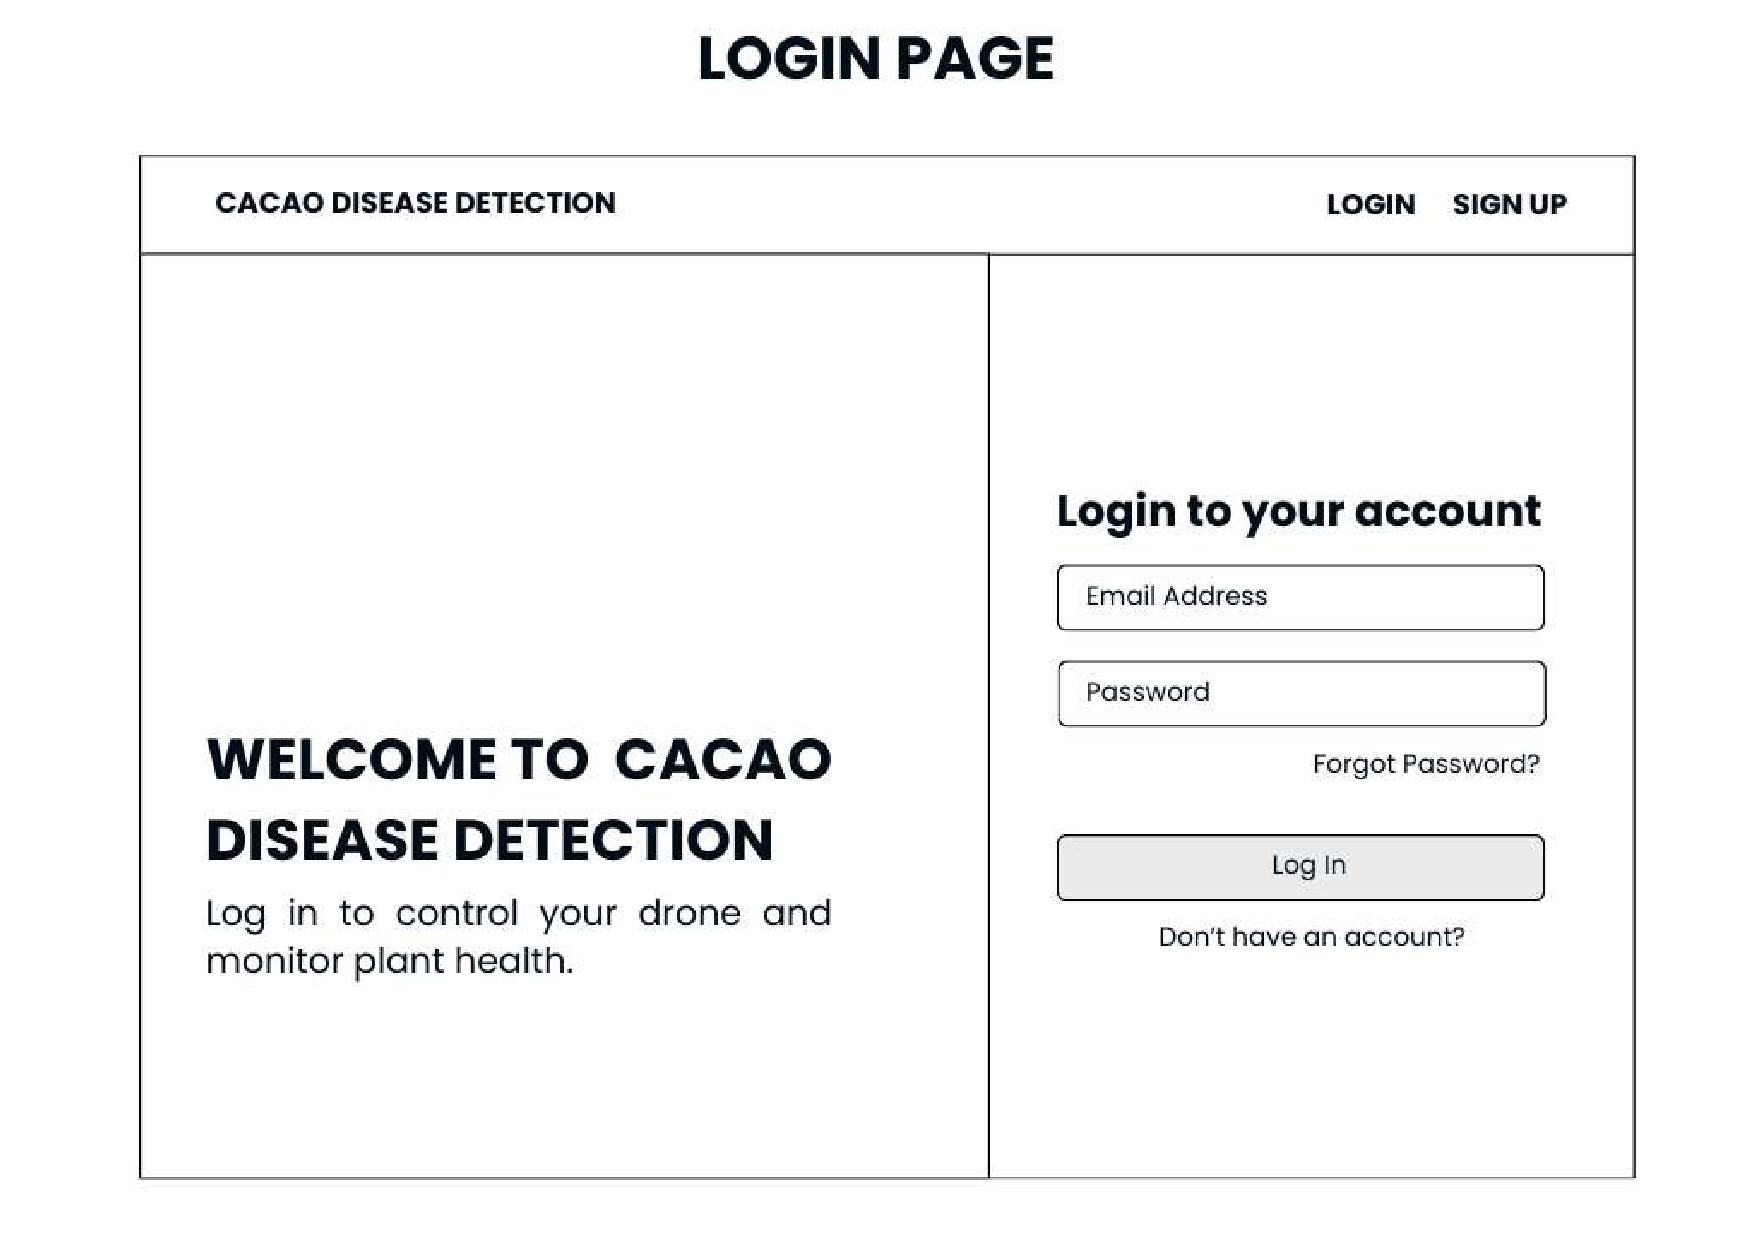
\includegraphics[width=0.7\textwidth]{figures/Login.pdf}
\end{figure}

Figure~\ref{fig:LoginGUI} shows the login page, which functions as the secure entry point to the system. It requires valid user credentials and integrates validation mechanisms to protect detection data. This security feature is essential for safeguarding sensitive agricultural information and ensuring that only authorized individuals can access UAV mission results.

\subsubsection*{Dashboard Page}

\begin{figure}[H]
	\centering
	\caption{Wireframe of Dashboard}
	\label{fig:DashboardGUI}
	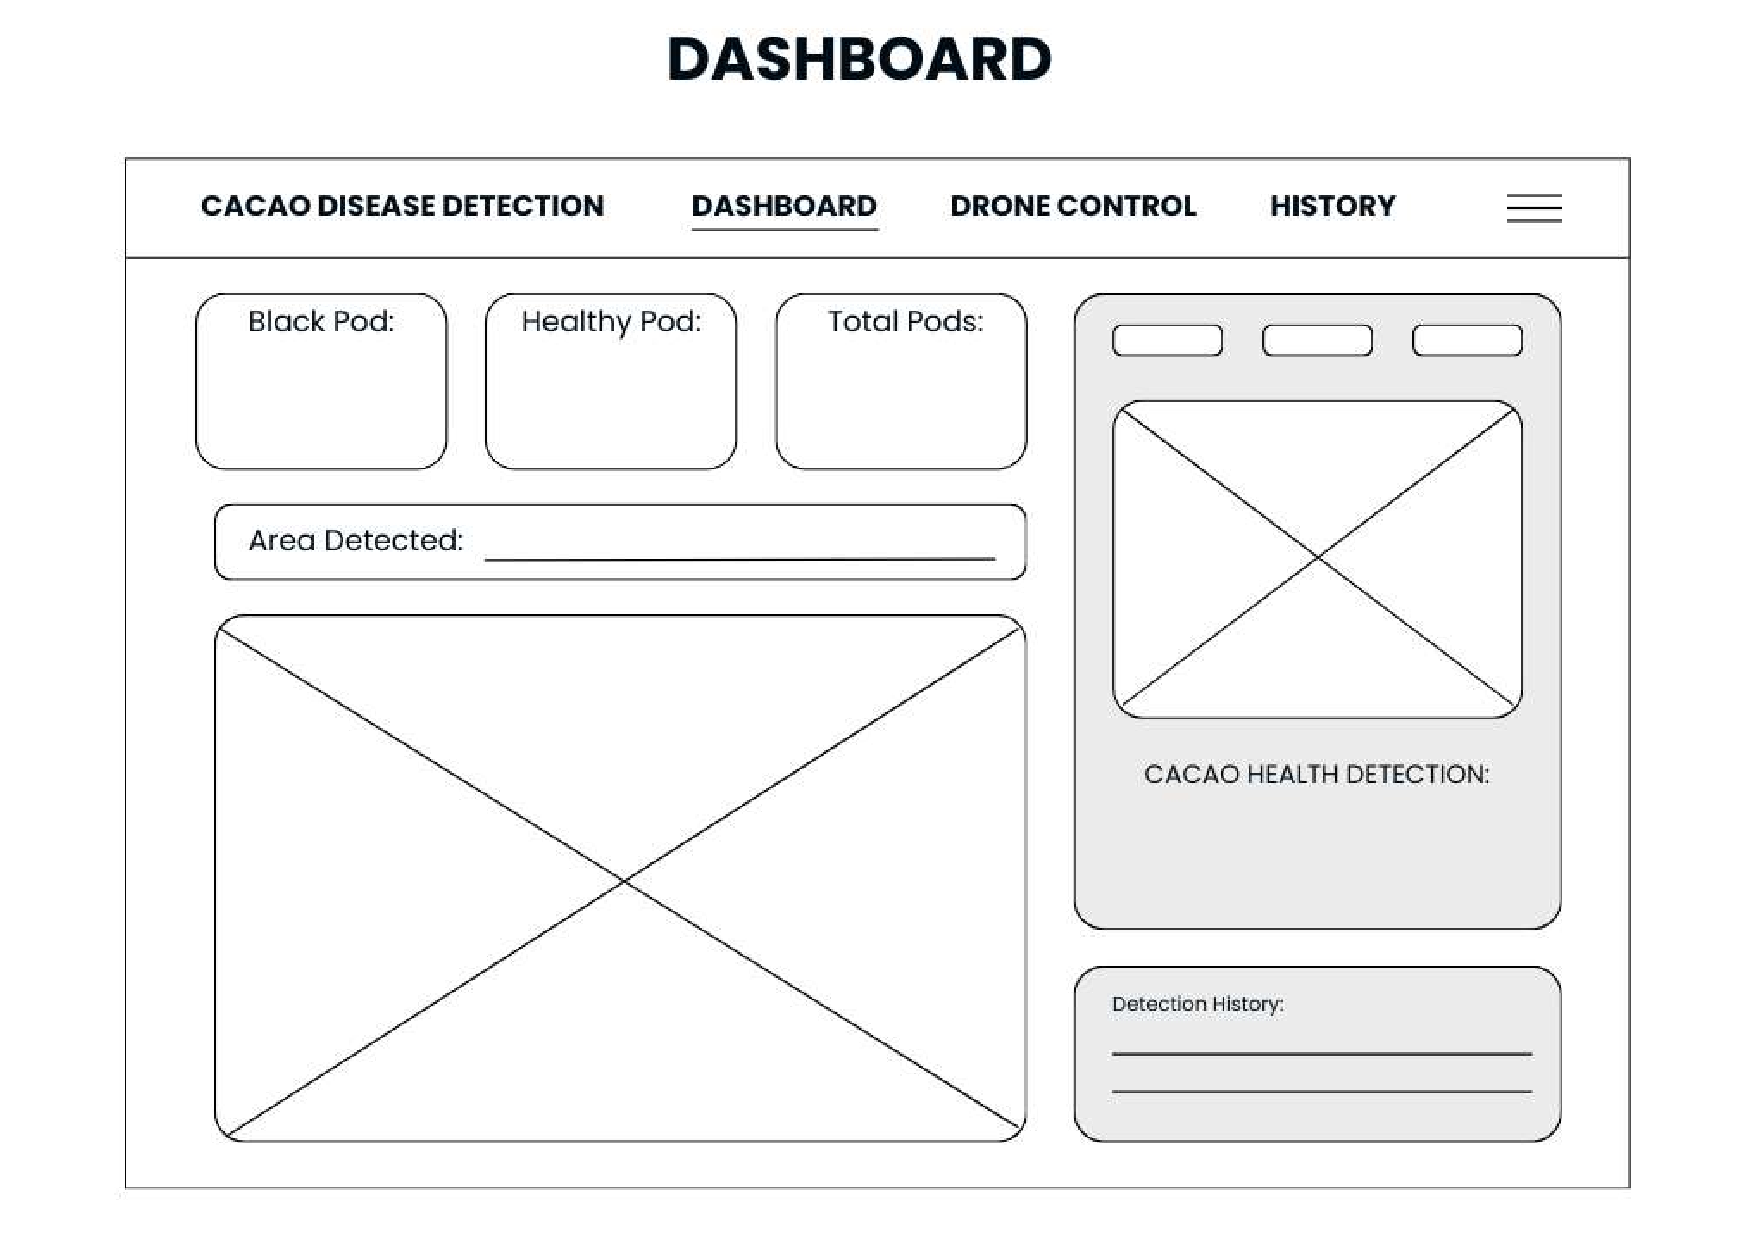
\includegraphics[width=0.9\textwidth]{figures/Dashboard.pdf}
\end{figure}

The dashboard, shown in Figure~\ref{fig:DashboardGUI}, serves as the central monitoring hub of the system. It provides real-time visualization of UAV detection outputs, including the number of healthy and infected cacao pods as identified by the YOLO model. This module directly supports the study’s aim of enabling farmers to quickly interpret crop conditions and make informed management decisions.

\subsubsection*{Drone Control Page}

\begin{figure}[H]
	\centering
	\caption{Wireframe of Drone Control}
	\label{fig:DroneControlGUI}
	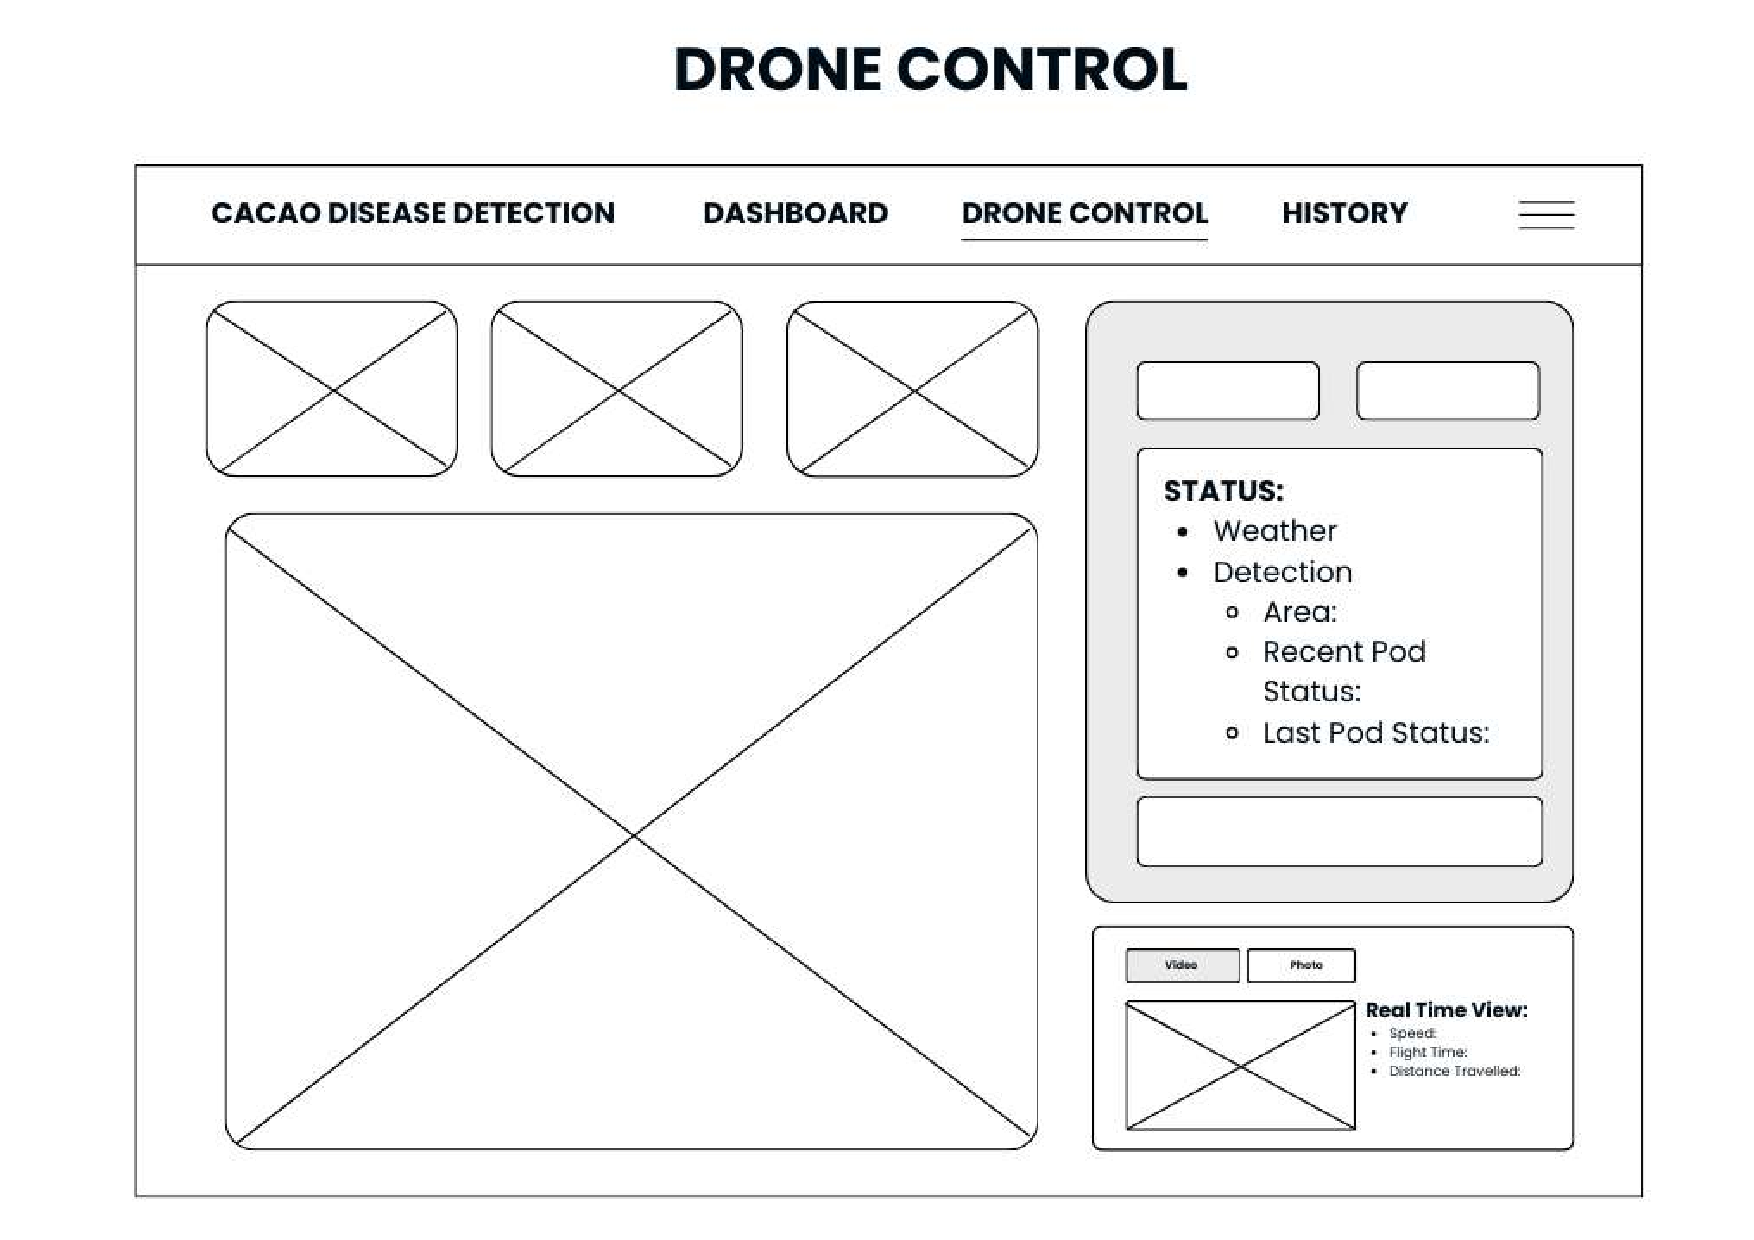
\includegraphics[width=0.9\textwidth]{figures/Drone Control.pdf}
\end{figure}

Figure~\ref{fig:DroneControlGUI} illustrates the drone control module, which enables operators to configure flight missions, issue commands, and monitor UAV status. By integrating UAV operations into the GUI, this page ensures that image acquisition for disease detection is efficient, systematic, and directly connected to the research workflow.

\subsubsection*{History Page}

\begin{figure}[H]
	\centering
	\caption{Wireframe of History Module}
	\label{fig:HistoryGUI}
	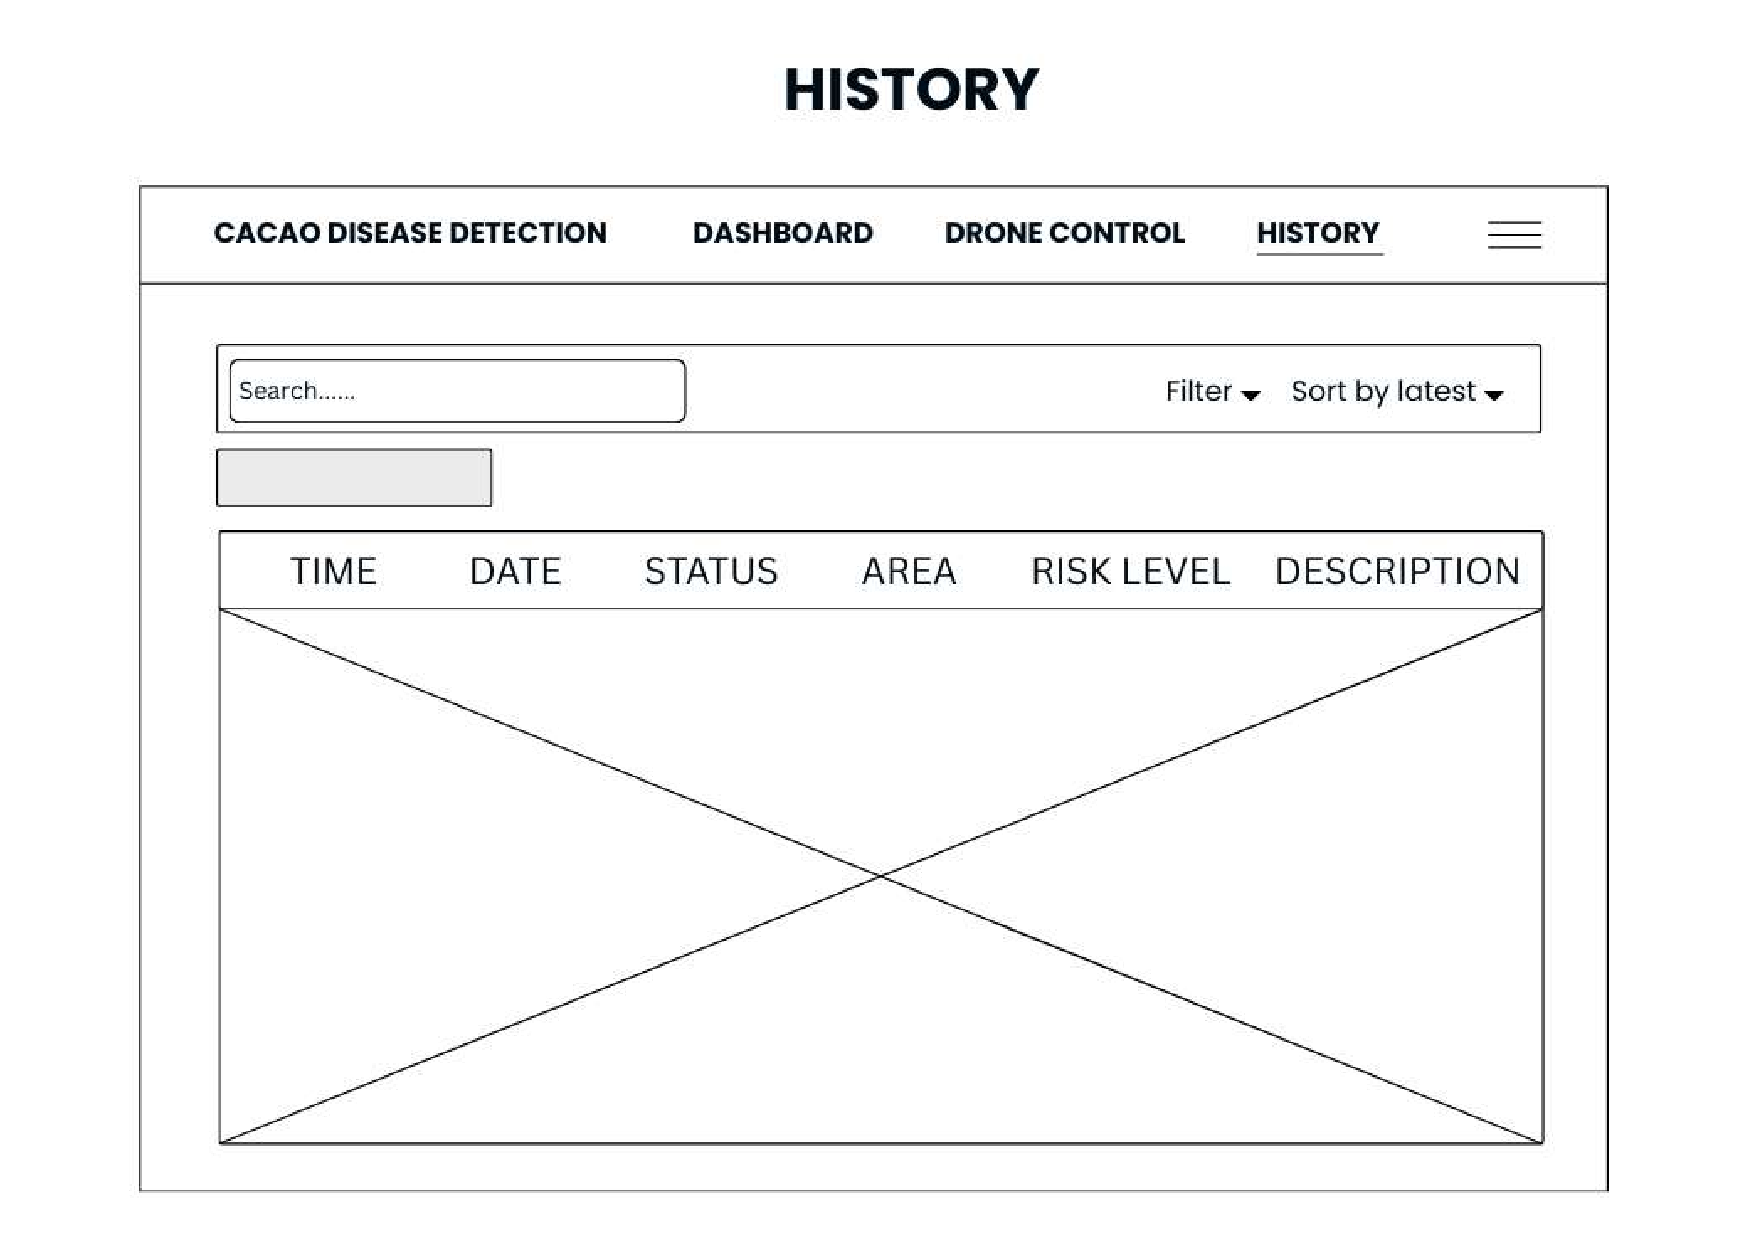
\includegraphics[width=0.9\textwidth]{figures/History.pdf}
\end{figure}

The history module, depicted in Figure~\ref{fig:HistoryGUI}, provides an archive of past detection missions and results. Users can browse, filter, and review earlier UAV detections, which supports long-term disease monitoring and analysis of crop health trends. This functionality reinforces the study’s goal of offering farmers a reliable tool for tracking disease progression and assessing the effectiveness of interventions.

\subsection*{YOLO-Based Detection Implementation}
YOLO (You Only Look Once) algorithm, a CNN-based object detection framework that employs Convolutional Neural Networks to simultaneously determine the location of objects within an image and classify them. Unlike traditional image classification models, which merely indicate the presence of an object, YOLO predicts both what the object is and where it is situated by drawing bounding boxes around it in a single processing step.

\begin{figure}[H]
	\centering
	\caption{Architecture of YOLOv11, showing backbone with new C3K2 blocks, attention modules (C2PSA), Spatial Pyramid Pooling Fast (SPFF), and multi-scale detection heads (adapted from Khanam and Hussain, 2024)}
	\label{fig:yolov11_architecture}
	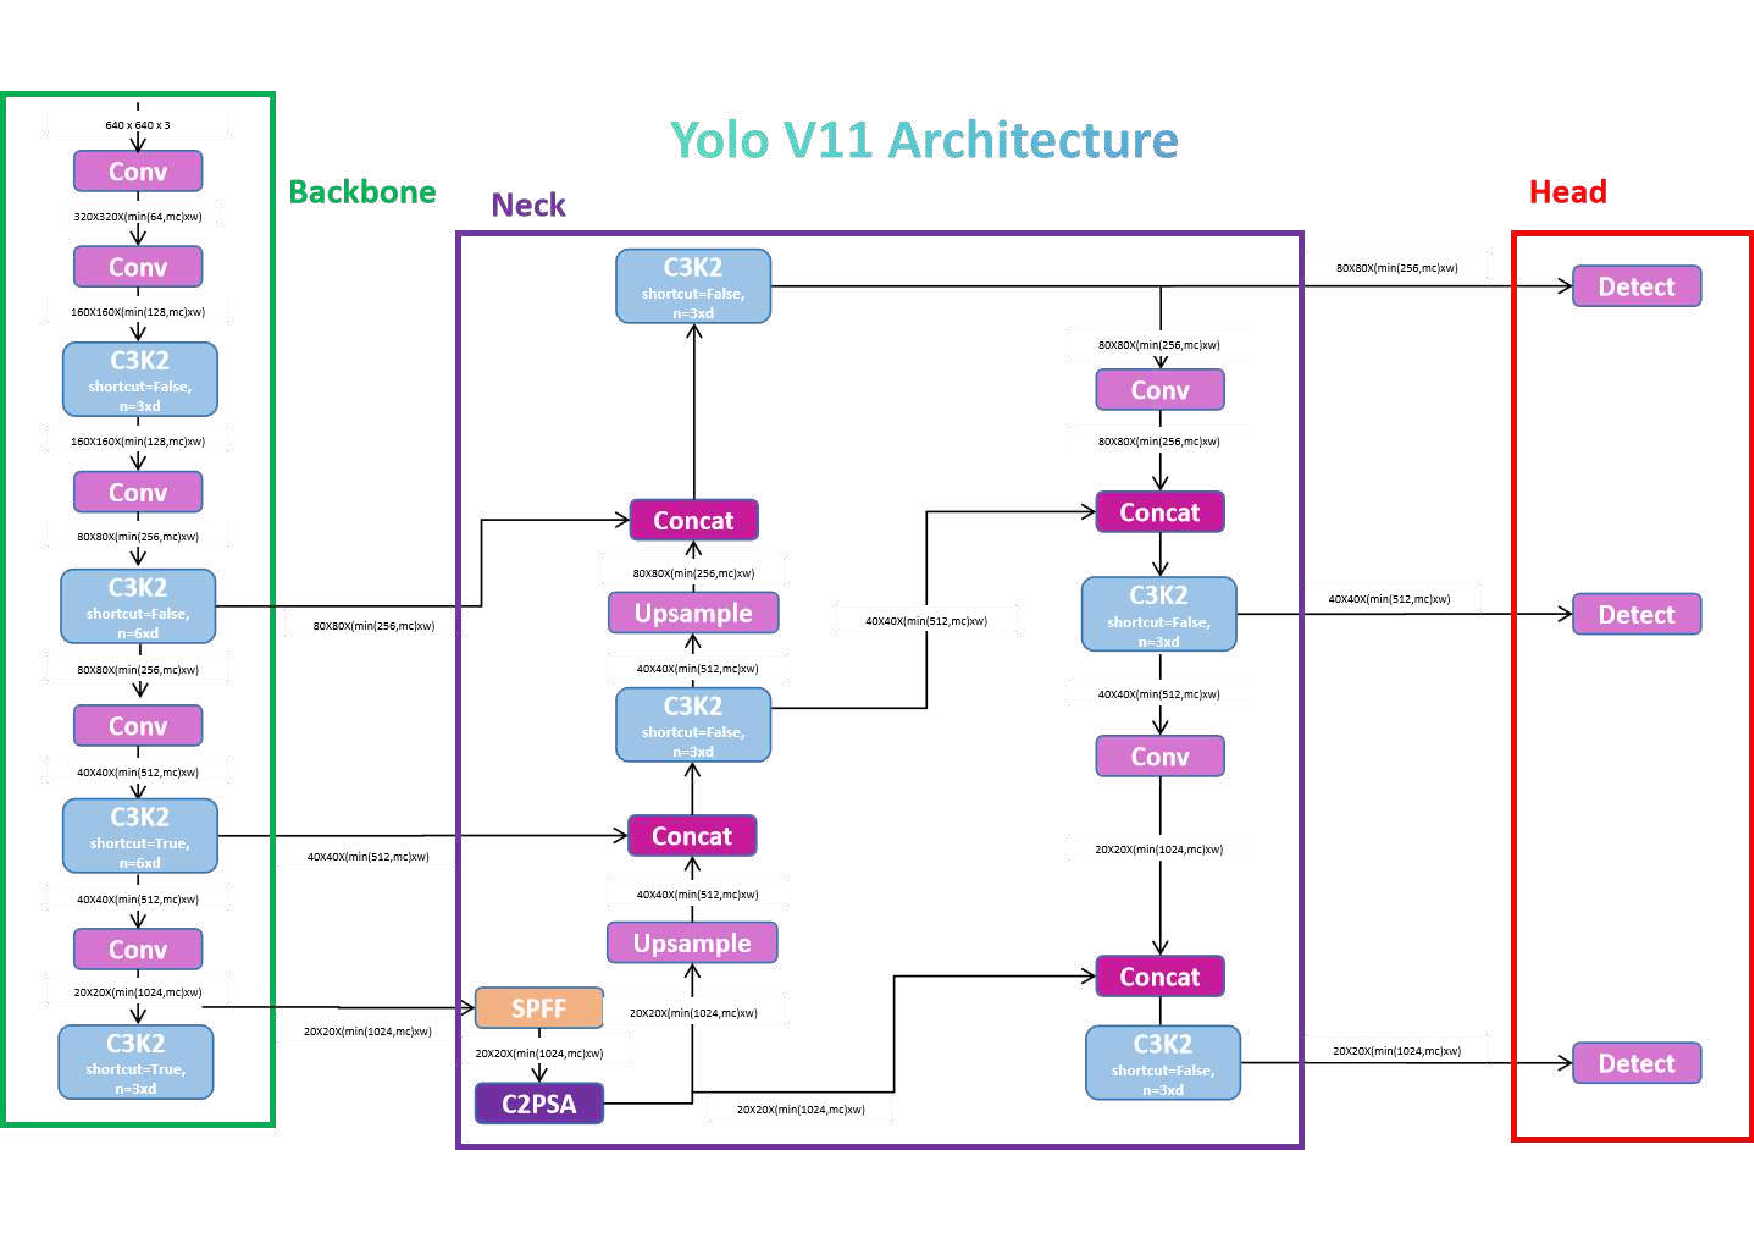
\includegraphics[width=0.9\textwidth]{figures/yolov11.pdf}
\end{figure}

YOLOv11 is employed since it introduces architectural improvements in feature extraction, particularly for small-object detection, and achieves higher accuracy with fewer parameters compared to earlier versions. YOLOv11 also provides scalable model variants that allow researchers to balance accuracy and computational requirements, making it highly suited for UAV-captured aerial imagery where cacao pods may appear small, numerous, and partially obscured. Figure~\ref{fig:yolov11_architecture} shows the  backbone for feature extraction, the neck for aggregating multi-scale feature maps, and the detection head outputs used for classifying and locating objects at various scales.

\noindent \textbf{Dataset Collection Method}

The dataset for this study will consist of both a custom dataset and external sources to ensure diversity and robustness. A custom dataset will be generated using images captured by a DJI RoboMaster TT’s built-in camera during scheduled flights over cacao plantations. Capturing images from multiple angles and altitudes will enhance the comprehensiveness and reliability of the dataset. In addition, publicly available image datasets such as those from Kaggle will be incorporated to supplement the collected data and increase variability. To ensure the model performs well in diverse real-world conditions, the combined dataset will include images of both healthy and diseased cacao pods under different lighting conditions, weather scenarios, and backgrounds. Special attention will be given to capturing multiple stages of infection and varying degrees of pod visibility. All images will be manually annotated to label regions of interest, which is essential for the supervised training of the YOLO model.

\subsection*{Data Preprocessing}

Before training and detection, the collected dataset will undergo a series of preprocessing steps to ensure consistency, quality, and suitability for the YOLOv11 model. First, UAV-captured videos are converted into individual frames at fixed intervals, with blurry or otherwise low-quality frames removed to reduce noise. Images, including those from external sources such as Kaggle, will be resized in accordance with YOLOv11's \texttt{imgsz} parameter to maintain a consistent input dimension while preserving the aspect ratio. Pixel values will be normalized (e.g., scaled to a [0,1] range or adjusted using mean and standard deviation) to aid convergence during training.

The dataset will be divided into training, validation, and testing subsets (commonly 70\% / 20\% / 10\%), ensuring that class distributions (healthy vs. diseased) are preserved and preventing data leakage. Data augmentation will be applied to the training portion only, using transformations such as random flips, rotations, brightness/contrast adjustments, and possibly random crops, to enhance the model’s robustness to real-world variability. Annotation files will be standardized to a YOLO-compatible format so that both custom and external images follow the same label scheme.


\begin{figure}[H]
	\centering
	\caption{Workflow of the YOLOv11-based cacao disease detection system, showing data preparation, model input, and classification outputs.}
	\label{fig:Data Preprocessing Workflow}
	\includegraphics[width=0.9\textwidth]{figures/data processing.pdf}
\end{figure}

The process begins with raw imagery collected through Unmanned Aerial Vehicles (UAVs) and external datasets. The UAV-captured videos are converted into individual frames at fixed intervals, ensuring that every pod instance is represented across varying viewpoints. Blurry, redundant, or low-quality frames are systematically removed to eliminate noise and improve dataset consistency. The selected images are resized and normalized according to YOLOv11’s input dimensions (e.g., 640×640 pixels), preserving the aspect ratio to prevent geometric distortion. Normalization scales pixel values into a uniform range (typically 0–1) to enhance computational efficiency and model stability.

The curated dataset is then divided into training, validation, and testing subsets, often following a 70–20–10 ratio. This split ensures balanced class representation and prevents overfitting by maintaining a consistent ratio of healthy and diseased pods across subsets. Data augmentation is applied exclusively to the training set to simulate real-world variability and improve the model’s generalization. Transformations such as random horizontal and vertical flips, rotations, brightness and contrast adjustments, and cropping expose the model to different illumination, orientation, and scale conditions. All annotations are standardized into the YOLO label format, which specifies object class IDs and bounding box coordinates in normalized values. This standardized structure ensures seamless integration with YOLOv11’s training and detection pipeline, enabling the model to correctly interpret positional and categorical information during learning.


\subsection*{Cacao and Disease Detection}

The UAV-captured cacao images are fed into the YOLOv11 model for automated object detection and disease classification. YOLOv11 divides each image into a predefined grid structure, where each grid cell predicts multiple bounding boxes, corresponding confidence scores, and class probabilities. This design allows the model to simultaneously identify multiple cacao pods within a single frame, accurately localizing each pod even under challenging conditions such as dense foliage, overlapping objects, or inconsistent lighting. Detected pods are enclosed within bounding boxes that represent the system’s prediction of their exact position within the image.


Once localization is complete, YOLOv11 proceeds with the classification of each detected pod as either healthy or infected with black pod disease. This classification is based on visual patterns learned during model training, including texture irregularities, surface discoloration, dark lesions, and other symptoms characteristic of infection. The model leverages deep feature extraction through its backbone network, multiscale feature fusion in the neck, and final detection through its head architecture. The output consists of annotated images displaying bounding boxes and class labels, where healthy pods are distinctly marked from diseased ones. This end-to-end workflow enables precise, efficient, and scalable cacao pod monitoring, facilitating early detection and management of black pod disease in agricultural environments.


\subsection*{Visual and Object Geo-localization}

The UAV is equipped with a GPS module and a downward-facing camera that captures images of the cacao trees during flight. Each image is associated with the DJI RoboMaster TT’s geospatial position $(\text{L}at_d, \text{L}on_d, \text{A}lt_d)$ at the moment of capture. The images are then processed using an object detection model (YOLOv11), which generates bounding boxes around identified cacao trees. A bounding box is defined by its pixel coordinates $(x, y, w, h)$, where $(x, y)$ is the top-left corner, and $w$ and $h$ are the width and height in pixels.

To estimate the ground location of each detected cacao tree, the relative position of the bounding box within the image plane is linked to the UAV’s GPS coordinates, as illustrated in Figure~\ref{fig:tree}.

\begin{figure}[H]
	\centering
	\caption{Tree Geo-localization}
	\label{fig:tree}
	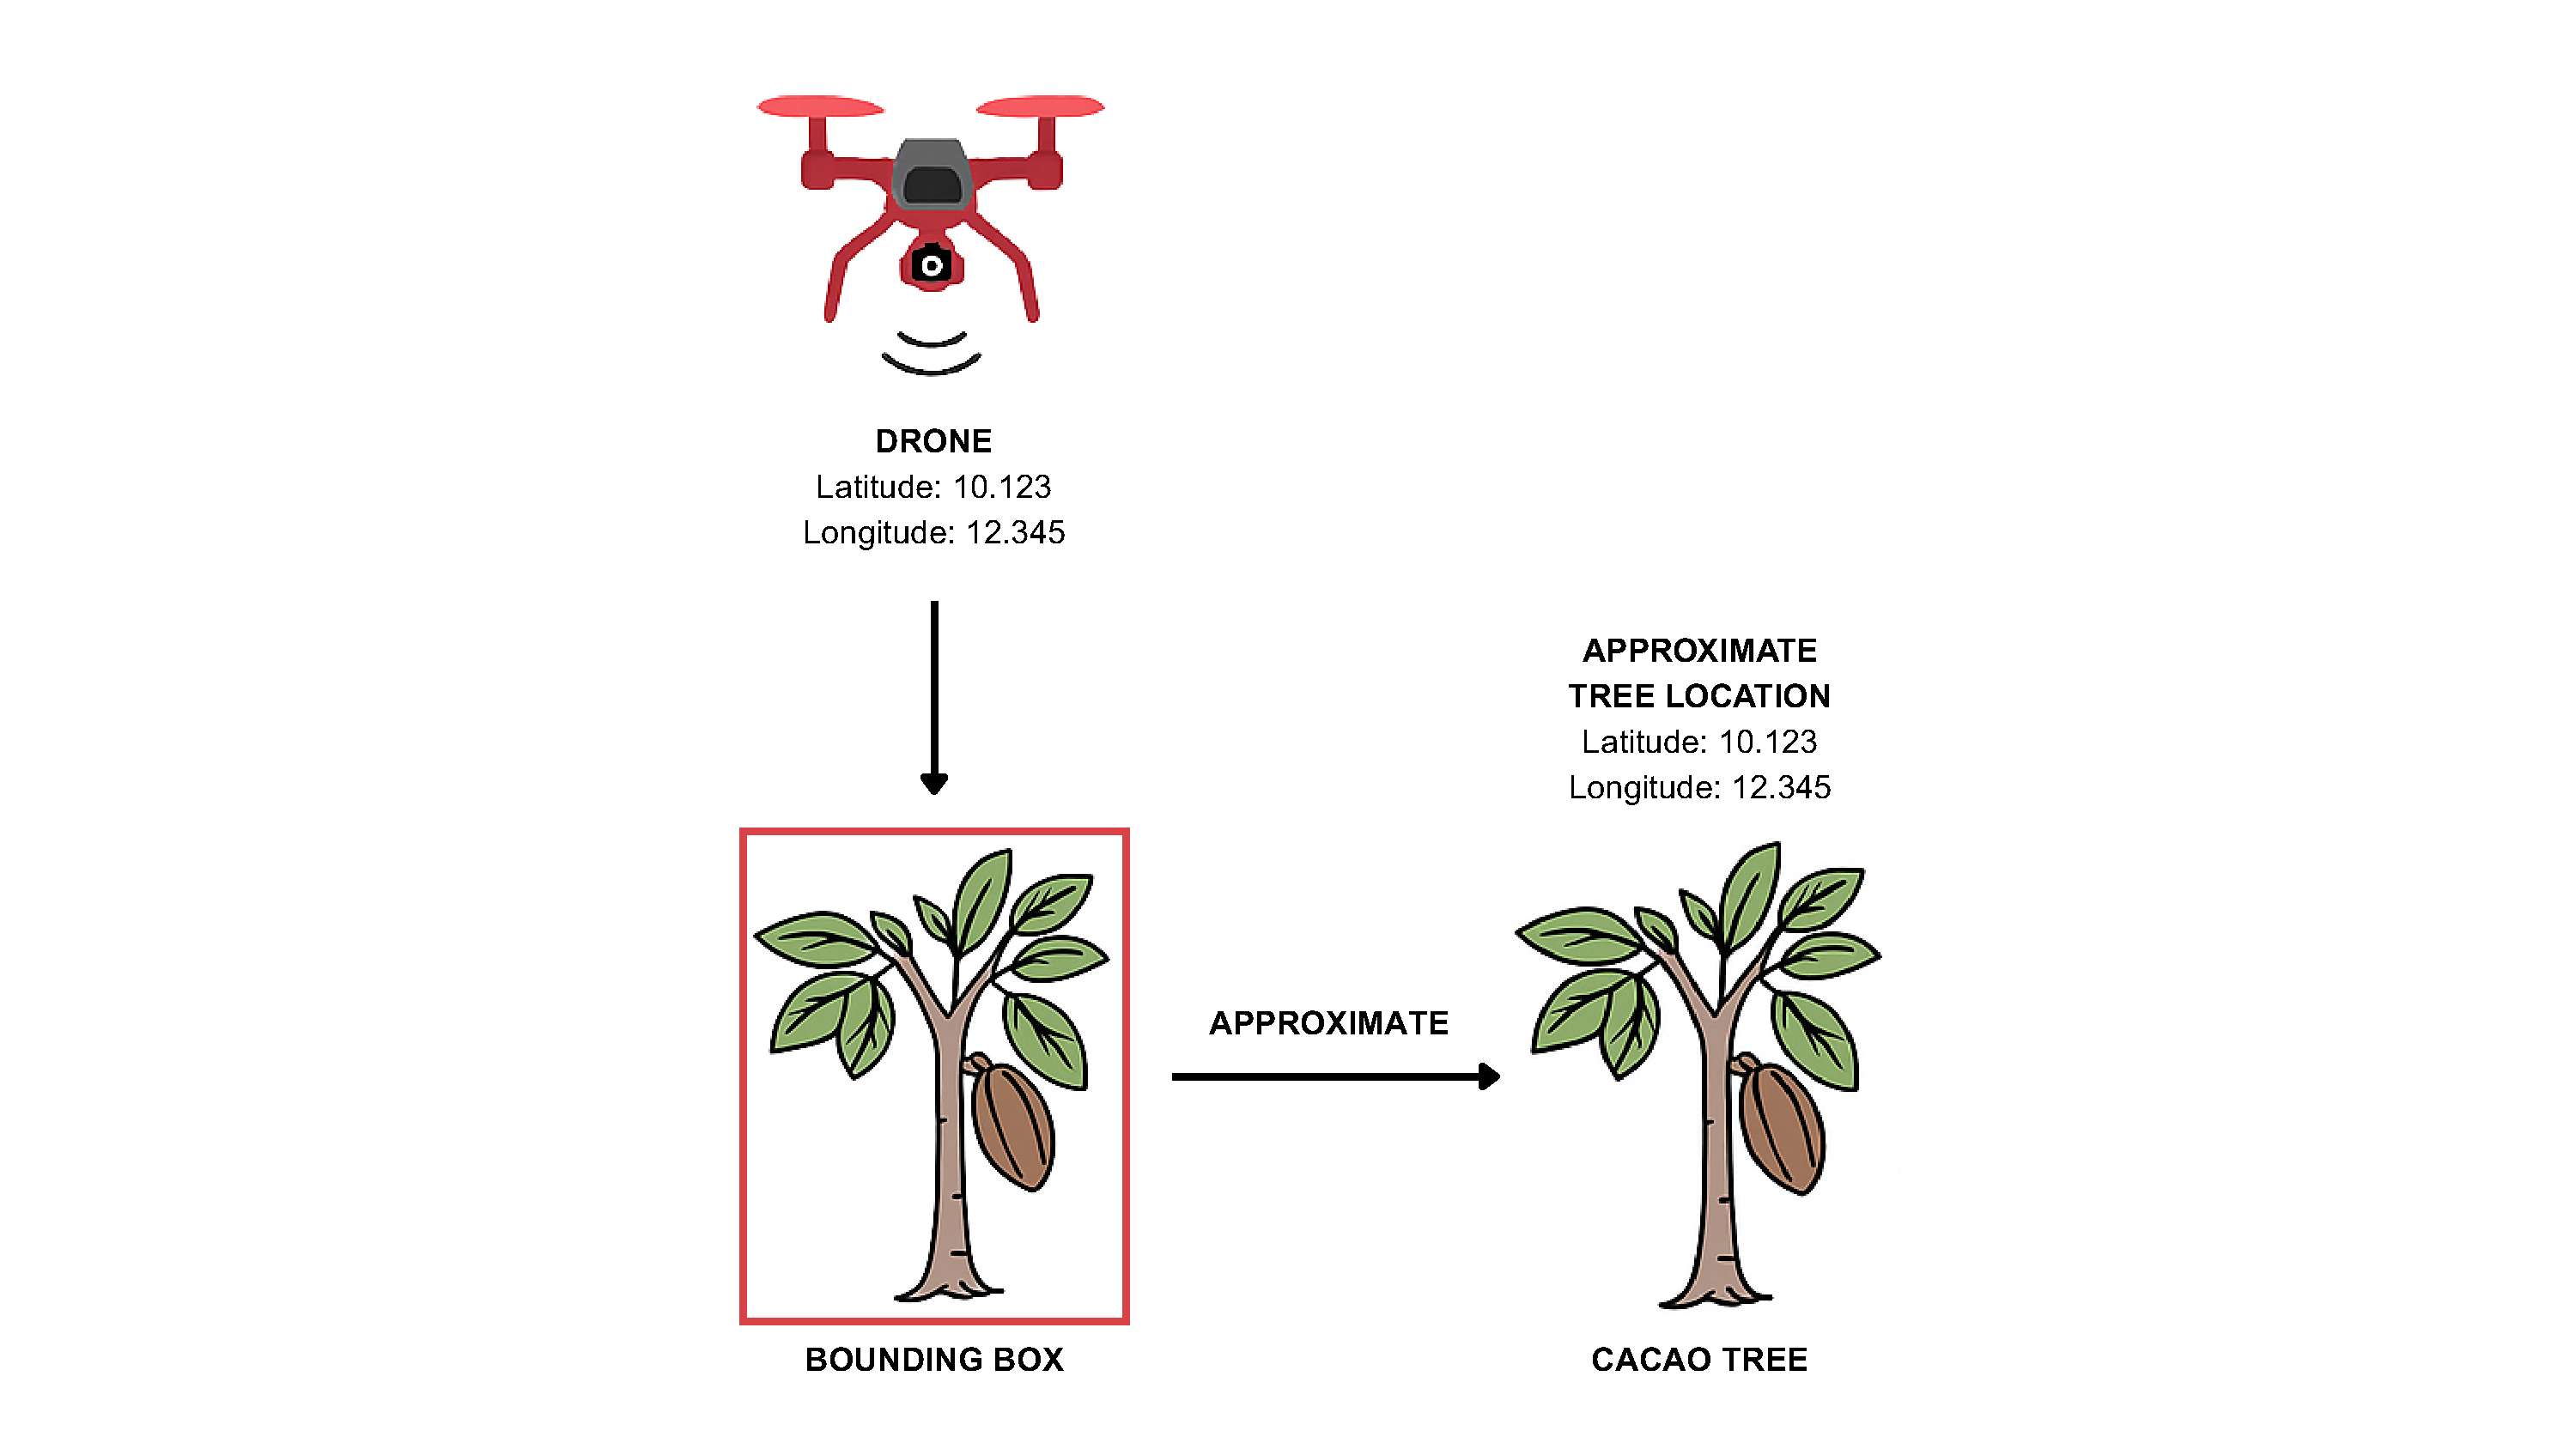
\includegraphics[width=0.9\textwidth]{figures/Tree Geolocalization.pdf}
\end{figure}

In Figure-\ref{fig:treex}, the size of the bounding box provides an indication of the distance between the drone and the trees: larger bounding boxes imply closer proximity, while smaller bounding boxes indicate greater distance.

\begin{figure}[H]
	\centering
	\caption{Bounding box as Proximity indicator}
	\label{fig:treex}
	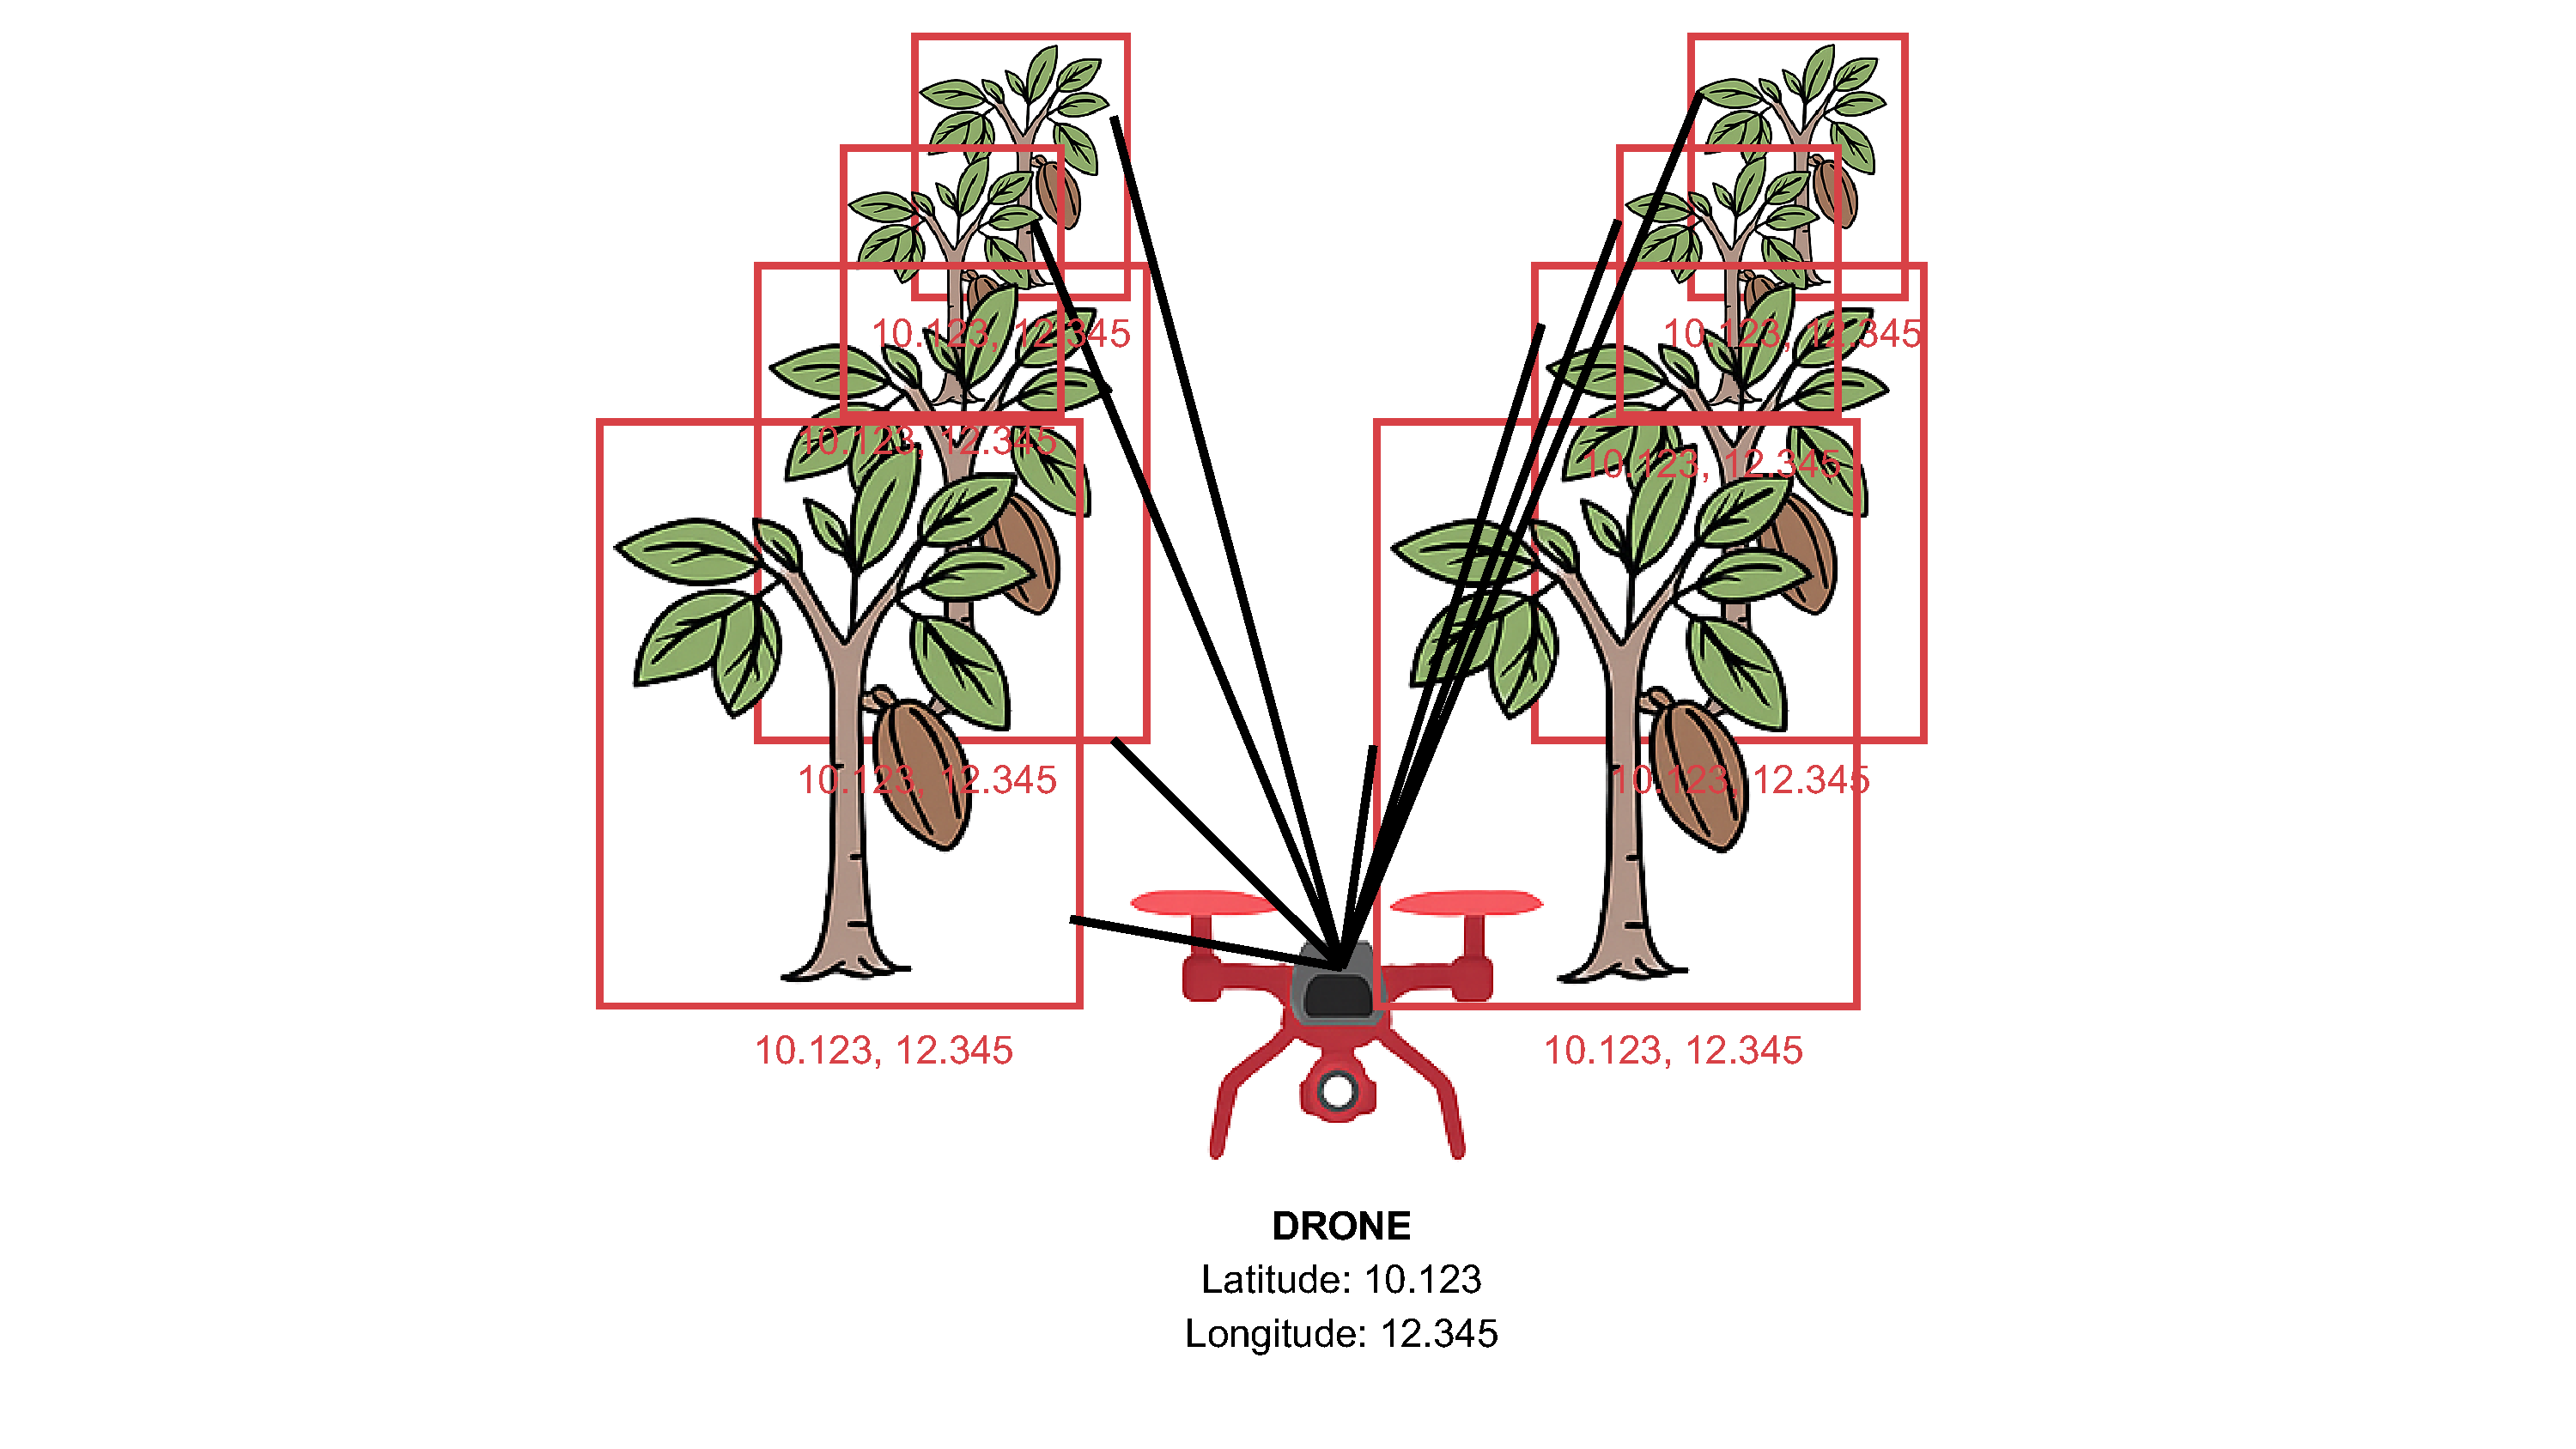
\includegraphics[width=0.9\textwidth]{figures/Bounding box as a Proximity Indicator.pdf}
\end{figure}

Following the approach of Liqun Ma et al., landmarks (objects with known real-world heights) are detected and tracked, and geometric similarity relations are used. The normalized bounding box size is defined as:
\begin{equation}
	S_\text{norm} = \frac{w \cdot h}{W \cdot H},
\end{equation}
where $W$ and $H$ are the width and height of the captured image in pixels. $S_\text{norm}$ serves as a proxy for the relative closeness of the tree.

Given the altitude of the UAV, the Ground Sampling Distance (GSD) is computed to determine the real-world size represented by one pixel:
\begin{equation}
	\text{GSD} = \frac{\text{SensorWidth} \cdot \text{Altitude}}{\text{FocalLength} \cdot W},
\end{equation}
where \text{SensorWidth} is the physical width of the camera sensor, \text{FocalLength} is the lens focal length, and $W$ is the width of the image in pixels. Nex and Romondino suggested that the bounding box size in meters can be approximated as:
\begin{equation}
	S_\text{m} = w \cdot \text{GSD}.
\end{equation}

This enables the estimation of how far the tree is from the drone’s nadir point. The ground coordinates of the detected tree $(\text{L}at_t, \text{L}on_t)$ are then approximated by offsetting the drone’s GPS coordinates according to the relative position of the bounding box center in the image:

\begin{align}
	\Delta y & = \frac{y + \frac{h}{2} - \frac{H}{2}}{H} \cdot FOV_y \cdot Alt_d \\
	\Delta x & = \frac{x + \frac{w}{2} - \frac{W}{2}}{W} \cdot FOV_w \cdot Alt_d
\end{align}

where $FOV_x$ and $FOV_y$ are the horizontal and vertical fields of view of the camera. These offsets represent the horizontal distances on the ground in meters relative to the UAV’s nadir. They can then be converted into latitude and longitude shifts


\begin{align}
	\text{Lat}_t & = \text{Lat}_d + \frac{\Delta y}{R} \cdot \frac{180}{\pi}                          \\
	\text{Lon}_t & = \text{Lon}_d + \frac{\Delta x}{R \cdot \cos(\text{Lat}_d)} \cdot \frac{180}{\pi}
\end{align}

Through this process, each detected bounding box is translated from an image coordinate system into an approximate geospatial coordinate system. Larger bounding boxes correspond to smaller offsets and closer estimated tree positions, while smaller bounding boxes indicate greater distances from the UAV. This integration of bounding box detection and geo-referencing enables the creation of a plantation map, where cacao trees are marked along with their health status.


\subsection*{UAV Drone System}

\begin{figure}[H]
	\centering
	\caption{DJI RoboMaster TT UAV}
	\label{fig:robomaster_tt}
	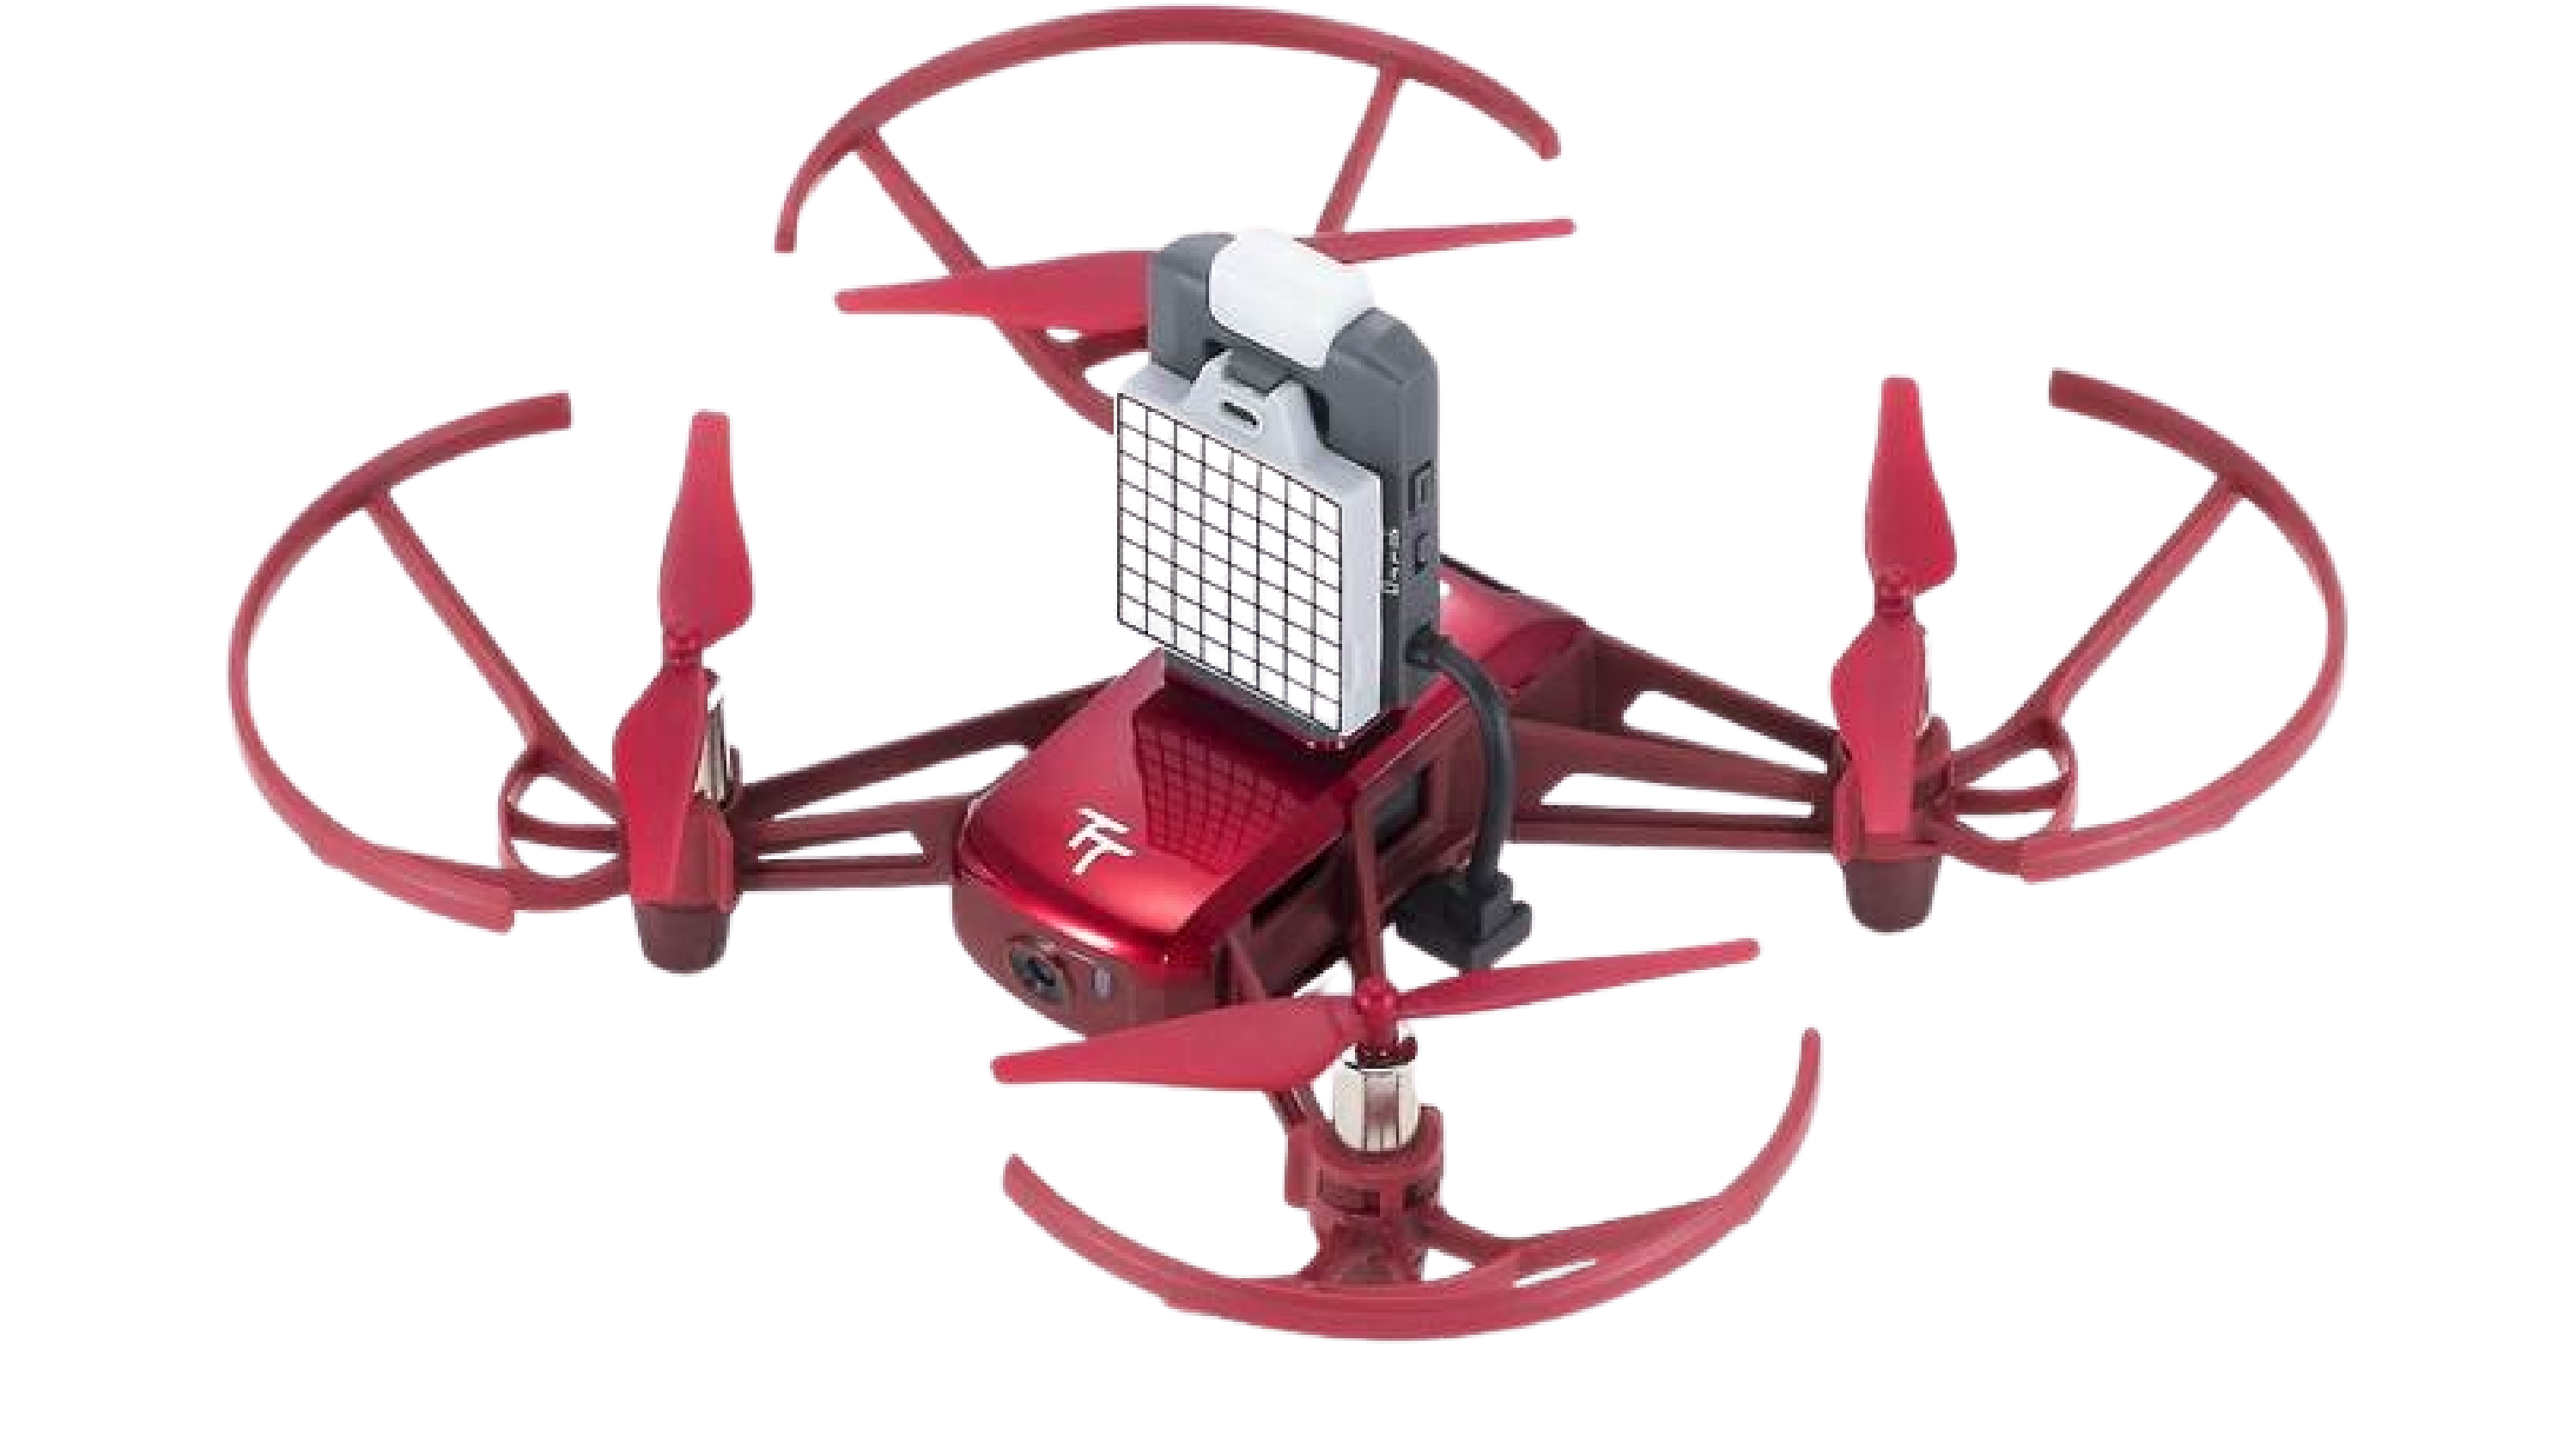
\includegraphics[width=0.5\textwidth]{figures/Robomaster_TT.pdf}
\end{figure}


The DJI RoboMaster TT (Tello Talent), a programmable quadcopter
equipped with a Vision Positioning System, a 5 MP camera, and an expansion kit for modular extensions.
It was chosen for its lightweight design, stability at low altitudes, and compatibility with open-source
programming platforms.

The RoboMaster TT integrates several important functions. Its flight system combines a flight controller
and propulsion motors with the Vision Positioning System (VPS), which uses a downward-facing camera and
infrared sensors to maintain stable hovering at low altitudes without relying on GPS. This feature is
essential for operating indoors or close to the ground, such as at eye level within cacao plantations.
The onboard 5 MP camera enables the capture of still images and 720p HD video, suitable for documenting
cacao pods. Power is supplied by a 3.8 V, 1100 mAh LiPo battery, supporting flight times of up to
13 minutes. Safety features include propeller guards, battery protection, and automatic landing in case
of weak signals or low power. The expansion kit includes an ESP32-based open-source controller, providing
UART, I2C, GPIO, PWM, and SPI interfaces for integrating additional modules such as the GPS receiver.

\subsection*{Command-based Mission Control with RoboMaster TT SDK}
The Software Development Kit (SDK) enables command-based mission planning with the
DJI RoboMaster TT. Through the SDK, the drone executes scripted flight commands such as
\texttt{takeoff}, \texttt{forward(x)}, \texttt{back(x)}, \texttt{cw(angle)}, and \texttt{land},
allowing it to follow predefined flight paths across cacao rows. During these missions, the drone
captures images of cacao pods at specific intervals, paired with location data provided by the
integrated NEO-M8N GPS module.

An offline detection approach was adopted: the collected images and GPS coordinates are stored
and later processed using the YOLO algorithm. The results of detection are then mapped in QGIS
to identify and visualize areas affected by \textit{Phytophthora palmivora}. This workflow
synchronizes drone navigation, image acquisition, and geotagging while accounting for the
hardware limitations of the RoboMaster TT.

\subsection*{GPS Integration and Data Handling}
A NEO-M8N GPS module was connected to the open-source controller via UART for geolocation.
The NEO-M8N is a high-performance GNSS receiver capable of tracking multiple satellite systems
(GPS, GLONASS, Galileo, and BeiDou). It provides accurate position, velocity, and time data,
which were synchronized with each captured image to create geotagged datasets. This integration
enabled the precise mapping of cacao pods and potential disease symptoms in QGIS.

All communications between the UAV and the ground station were established through a
Wi-Fi connection. The SDK relies on UDP packets transmitted over Wi-Fi to send
flight commands and receive status updates. For structured telemetry such as GPS coordinates
and mission logs, the MQTT protocol was integrated as a lightweight messaging layer,
ensuring reliable delivery of small data packets. Image files, due to their larger size, were
transferred directly via the Wi-Fi link to the ground station.

After each mission, the drone transmitted images and GPS logs to a central database.
The ground station retrieved these records from the database for preprocessing
and analysis. This workflow ensured that raw images and geospatial metadata were securely
stored and easily accessible for the YOLO-based detection system and subsequent
spatial visualization in QGIS.

\subsection{Telemetry Overlay}

During flight, the UAV continuously records telemetry data consisting of timestamp, latitude, longitude, altitude, and orientation parameters (yaw, pitch, and roll). These telemetry values are synchronized with the video stream and image frames, ensuring that every recorded frame has an associated spatiotemporal context.

\begin{figure}[H]
	\centering
	\caption{Telemetry Overlay}
	\label{fig:telemetry_overlay}
	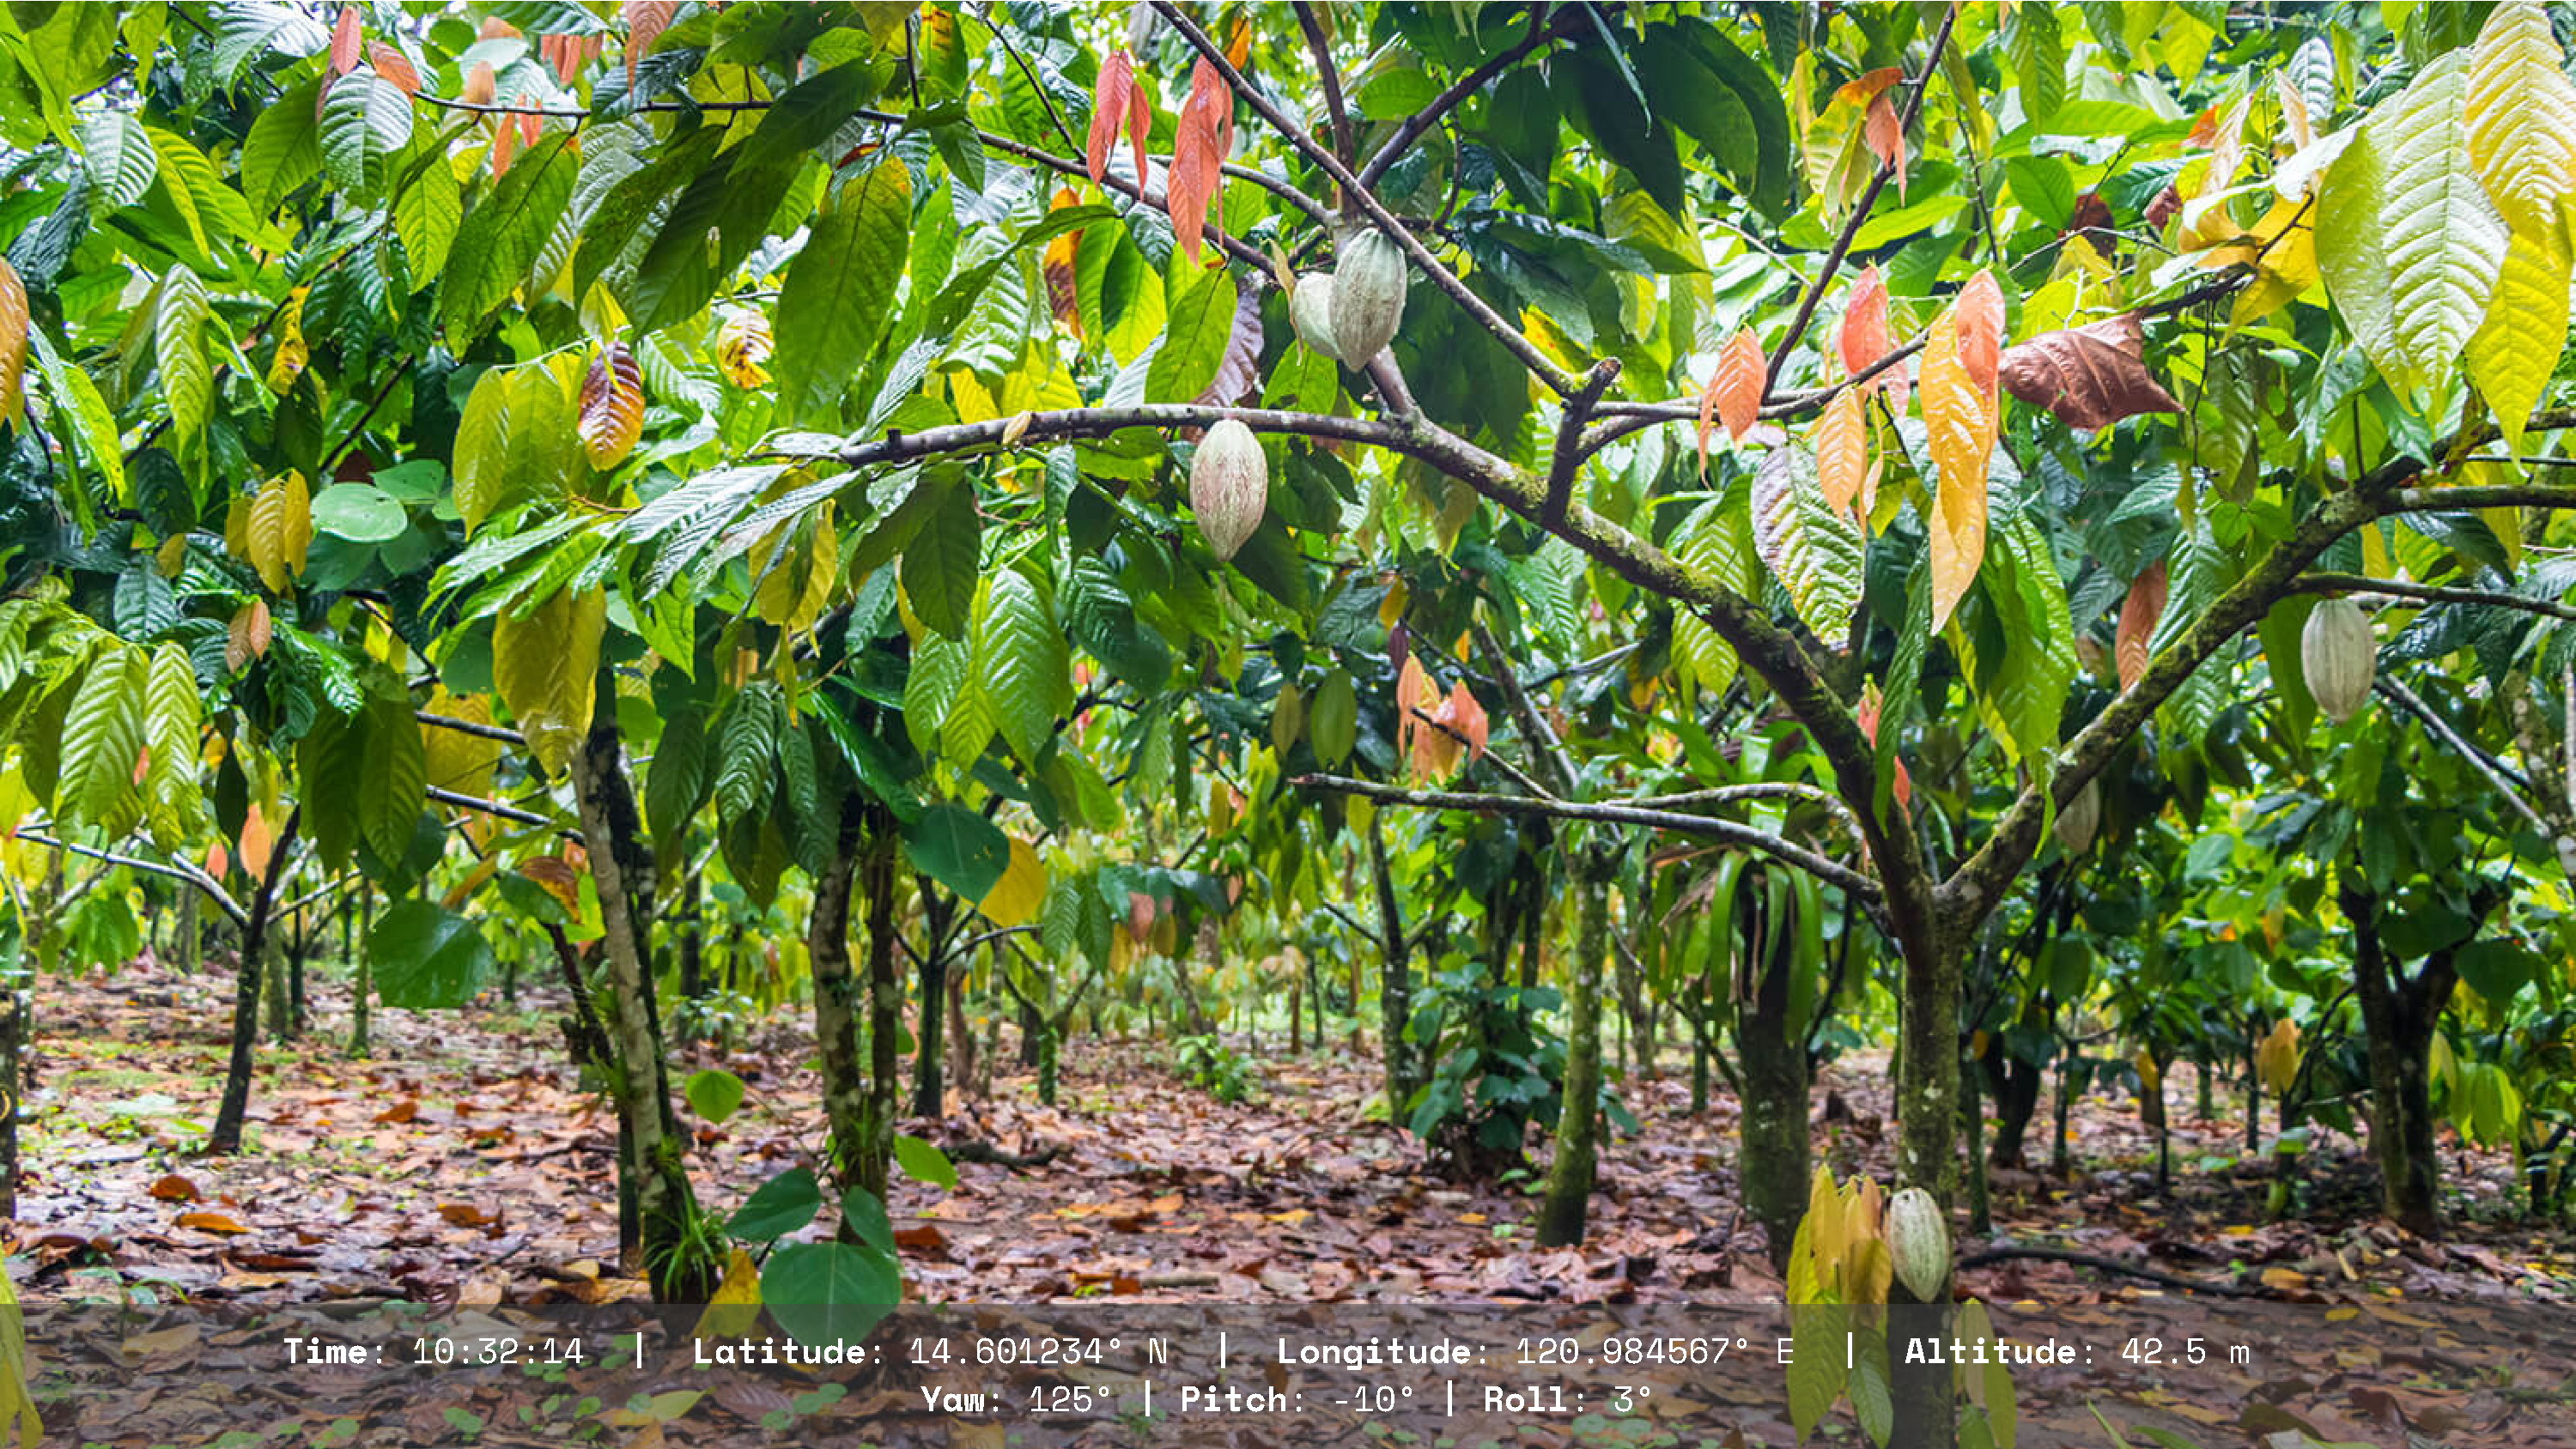
\includegraphics[width=0.9\textwidth]{figures/Telemetry.pdf}
\end{figure}

Telemetry overlay, as shown in Fig.~\ref{fig:telemetry_overlay}, refers to the process of superimposing flight data directly onto the visual feed or processed image output. This provides operators with real-time situational awareness and enables more precise post-flight analysis. Telemetry overlay displays the UAV’s recording time, positional coordinates, altitude, and orientation alongside the YOLOv11 bounding boxes of detected cacao trees. This integration ensures that detections are not only localized within an image but also connected to the UAV’s position and state during capture.

The inclusion of telemetry information serves multiple functions.
(1) The timestamp allows for chronological indexing of detections, supporting analysis of cacao disease monitoring.
(2) The geographic coordinates (latitude, longitude, altitude) provide a direct spatial reference to the UAV’s position during detection.
(3) The IMU-derived orientation (yaw, pitch, roll) supplies critical context on the UAV’s attitude, which can affect the angle and scale of captured images.

Together, these parameters create a transparent record of the flight path and its associated detections, enabling accurate mapping, post-flight analysis, and data validation.

\subsection{Materials and Cost}

\begin{longtable}{p{8cm} r}
	\caption{\textit{Components and Cost}} \label{tab:components} \\

	\toprule
	\textbf{Component}        & \textbf{Price (₱)}                \\
	\midrule
	\endfirsthead

	\toprule
	\textbf{Component}        & \textbf{Price (₱)}                \\
	\midrule
	\endhead

	\bottomrule
	\endfoot

	Drone (DJI RoboMaster TT) & 20,000.00                         \\
	NEO-M8N GPS module        & 300.00                            \\
	\midrule
	\textbf{Total Cost}       & \textbf{20,300.00}                \\
\end{longtable}


\section{Test and Evaluation}

Testing will be conducted to ensure that the system will operate accurately, efficiently, and be suitable for real-world use in cacao farm management. The process will involve functional testing, usability testing, and performance testing. Functional testing will verify whether key features such as UAV image capture, detection of Phytophthora palmivora-infected cacao pods using YOLO, and geotagging of infected trees perform as intended, with each function tested through defined inputs and expected outputs. Usability testing will assess how easily end users, particularly cacao farmers, can navigate and interact with the system by performing essential tasks such as logging in, accessing detection results, and interpreting geotagged maps. Feedback will be collected using the System Usability Scale (SUS) to evaluate the overall user experience. Performance testing will measure the system’s responsiveness and accuracy, focusing on the time taken from image capture to the display of results, as well as the efficiency in processing high-resolution images and managing data. Together, these tests will validate the system’s reliability, user-friendliness, and effectiveness in supporting early disease detection and timely intervention.

\subsection{Functional Testing}

Functional testing will be carried out to ensure that every part of the system will work as intended. This testing will begin once the prototype is complete. It will focus on verifying key features such as capturing images through the drone, detecting healthy and infected cacao pods using the YOLO, tagging infected trees’ locations with GPS, and displaying results clearly on the dashboard. Each function will be tested by providing specific inputs and checking if the outputs match the expected results.

\subsection{Usability Testing}

Usability testing will be conducted to make sure the system is easy and practical for cacao farmers to use. After the prototype is ready, farmers will be invited to try important features such as logging in, flying the drone, viewing pod detection results, and checking the map showing infected trees. After using the system, they will fill out a short survey called the System Usability Scale (SUS), which measures how user-friendly the system feels. The survey uses a rating scale from 1 to 5 and asks about how easy the system is to learn, how confident they feel using it, and whether the features work well together. Scores are converted to a total out of 100, with scores above 68 generally meaning the system is easy to use. This process will help the team understand what works well and what needs improvement before the system is fully deployed.
\pagebreak

\subsection*{Performance Testing}

\begin{longtable}{p{4cm} >{\centering\arraybackslash}p{7cm}}
	\caption{\textit{Performance Metrics for Cacao Pod Detection}} \label{tab:metrics}                    \\
	
	\toprule
	\textbf{Metric} & \textbf{Equation}                                                                   \\
	\midrule
	\endfirsthead
	
	\toprule
	\textbf{Metric} & \textbf{Equation}                                                                   \\
	\midrule
	\endhead
	
	\bottomrule
	\endfoot
	
	Accuracy        &
	$\displaystyle \frac{TP + TN}{TP + TN + FP + FN}$                                                     \\ \addlinespace \addlinespace
	
	Precision       &
	$\displaystyle \frac{TP}{TP + FP}$                                                                    \\ \addlinespace \addlinespace
	
	Recall          &
	$\displaystyle \frac{TP}{TP + FN}$                                                                    \\ \addlinespace \addlinespace
	
	F1-Score        &
	$\displaystyle \frac{2 \cdot \text{Precision} \cdot \text{Recall}}{\text{Precision} + \text{Recall}}$ \\ \addlinespace \addlinespace
	
	Error Rate      &
	$\displaystyle \frac{FP + FN}{TP + TN + FP + FN}$                                                     \\ \addlinespace \addlinespace
\end{longtable}

Performance testing will be conducted to evaluate the system’s responsiveness, accuracy, and overall reliability based on its core functionalities. This will include measuring the accuracy of detecting Phytophthora palmivora infected cacao pods using the YOLO, assessing the precision of geolocation through the GPS module and QGIS, and recording the system’s response time from image capture to the display of results on the dashboard. The testing will also evaluate the system using standard performance metrics such as Accuracy, Precision, Recall, F1-Score, and Error Rate to determine the effectiveness of the detection model. These evaluations will verify whether the system will meet its intended performance criteria and will be capable of supporting timely and informed decision-making in cacao disease management.

\begin{longtable}{p{4cm} >{\centering\arraybackslash}p{7cm}}
	\caption{\textit{Performance Metrics for Cacao Pod Detection}} \label{tab:metrics}                    \\

	\toprule
	\textbf{Metric} & \textbf{Equation}                                                                   \\
	\midrule
	\endfirsthead

	\toprule
	\textbf{Metric} & \textbf{Equation}                                                                   \\
	\midrule
	\endhead

	\bottomrule
	\endfoot

	Accuracy        &
	$\displaystyle \frac{TP + TN}{TP + TN + FP + FN}$                                                     \\ \addlinespace \addlinespace

	Precision       &
	$\displaystyle \frac{TP}{TP + FP}$                                                                    \\ \addlinespace \addlinespace

	Recall          &
	$\displaystyle \frac{TP}{TP + FN}$                                                                    \\ \addlinespace \addlinespace

	F1-Score        &
	$\displaystyle \frac{2 \cdot \text{Precision} \cdot \text{Recall}}{\text{Precision} + \text{Recall}}$ \\ \addlinespace \addlinespace

	Error Rate      &
	$\displaystyle \frac{FP + FN}{TP + TN + FP + FN}$                                                     \\ \addlinespace \addlinespace
\end{longtable}

Table~\ref{tab:metrics} presents the performance metrics used to evaluate the cacao pod detection system. Accuracy measures the overall correctness of the system by calculating the proportion of correctly classified instances, including both infected and healthy pods, out of the total number of samples. Precision indicates the proportion of pods identified as infected that are actually infected, which is important to minimize false positives. Recall measures the proportion of actual infected pods that the system correctly identifies, ensuring that most infected pods are detected. The F1-Score provides a balance between precision and recall by calculating their harmonic mean, which is particularly useful when both false positives and false negatives need to be minimized. 
